% =============================================================================
% methods.tex  -  Methods of Model3 = MarrowTwin (Model2 v1.0 + (N) a neutrophil chain with a
%                 post-mitotic storage pool and (P2) a platelet-specific suppression of MPP
%                 self-renewal by the CAR T - target signal)
% Tables and numbers come from Code/config.R via make_tables.R:
%   Rscript Methods/make_tables.R && latexmk -pdf methods.tex   (in Methods/)
% =============================================================================
\documentclass[11pt]{article}
\usepackage[a4paper,margin=2.2cm]{geometry}
\usepackage[T1]{fontenc}
\usepackage{lmodern}
\usepackage{microtype}
\usepackage{amsmath,amssymb}
\usepackage{booktabs}
\usepackage{array}
\usepackage{xcolor}
\usepackage{tikz}
\usetikzlibrary{arrows.meta,positioning,calc}
\usepackage[font=small,labelfont=bf]{caption}
\usepackage[round,authoryear]{natbib}
\usepackage[hidelinks]{hyperref}
% generated by make_tables.R from Code/config.R - do not edit
\newcommand{\valThapCentre}{2.71}
\newcommand{\valThapAimNadir}{0.537}
\newcommand{\valThapAimFour}{2.31}
\newcommand{\valKappaC}{1}
\newcommand{\valKappaCSd}{1}
\newcommand{\valThAm}{0.384}
\newcommand{\valThAmCal}{0.3839}
\newcommand{\valThAmSd}{1}
\newcommand{\valAmcTarget}{0.078}
\newcommand{\valAmcLdModelOne}{0.4}
\newcommand{\valAmcLdModelThree}{0.078}
\newcommand{\valNStructModelOne}{37}
\newcommand{\valNEstModelOne}{15}
\newcommand{\valNPopModelOne}{43}
\newcommand{\valNStructModelTwo}{39}
\newcommand{\valNEstModelTwo}{17}
\newcommand{\valNPopModelTwo}{45}
\newcommand{\valNFixedModelTwo}{22}
\newcommand{\valNStatesModelTwo}{27}
\newcommand{\valNParModelTwo}{41}
\newcommand{\valThal}{0.921}
\newcommand{\valCl}{0.156}
\newcommand{\valThalCal}{0.9207}
\newcommand{\valClCal}{0.1561}
\newcommand{\valAlcDayThirty}{0.848}
\newcommand{\valAncNadirAimFour}{0.221}
\newcommand{\valAncNadirModel}{0.019}
\newcommand{\valAncNadirDayModel}{2.75}
\newcommand{\valAncNadirModelTwo}{0.048}
\newcommand{\valAncNadirDayModelTwo}{2.25}
\newcommand{\valAncNadirModelOne}{0.22}
\newcommand{\valAncNadirDayModelOne}{5}
\newcommand{\valAncRecAimFour}{9.25}
\newcommand{\valAncRecModel}{9.25}
\newcommand{\valAncRecModelTwo}{9.25}
\newcommand{\valAmcNadirModel}{0.049}
\newcommand{\valAmcNadirDayModel}{1}
\newcommand{\valAncPreModelTwo}{0.65}
\newcommand{\valAncPreModel}{0.77}
\newcommand{\valAncLdModelTwo}{0.33}
\newcommand{\valAncLdModel}{0.46}
\newcommand{\valAncMidModelTwo}{0.42}
\newcommand{\valAncMidModel}{0.34}
\newcommand{\valKp}{0.3}
\newcommand{\valSrp}{0.21}
\newcommand{\valResP}{11.1}
\newcommand{\valGmax}{3}
\newcommand{\valGamma}{0.5}
\newcommand{\valGammaHi}{1}
\newcommand{\valGammaLo}{0.068}
\newcommand{\valGammaLimLo}{0.05}
\newcommand{\valGammaHiModelTwo}{2.2}
\newcommand{\valMttNLo}{0.68}
\newcommand{\valMttNHi}{15}
\newcommand{\valMttPlHi}{36.9}
\newcommand{\valMttMoHi}{11.1}
\newcommand{\valDzplLo}{-4}
\newcommand{\valDzplHi}{4}
\newcommand{\valDzplSd}{1}
\newcommand{\valEzPlLo}{0.018}
\newcommand{\valEzPlHi}{0.982}
\newcommand{\valHopf}{2.09}
\newcommand{\valHopfModelTwoChain}{2.37}
\newcommand{\valHopfOther}{2.37}
\newcommand{\valHopfOtherLineage}{megakaryocyte}
\newcommand{\valHopfMttHi}{1.10}
\newcommand{\valHopfMttHiModelTwo}{1.82}
\newcommand{\valBoxMaxRe}{-0.004}
\newcommand{\valPstar}{0.49}
\newcommand{\valEmax}{0.7}
\newcommand{\valEmaxSd}{1}
\newcommand{\valEmaxScreenSW}{0.7}
\newcommand{\valStructSd}{0.5}
\newcommand{\valEtaCentre}{1}
\newcommand{\valEtaSd}{1.2}
\newcommand{\valAlcTarget}{0.042}
\newcommand{\valRtol}{10^{-6}}
\newcommand{\valAtol}{10^{-9}}
\newcommand{\valHmax}{0.5}
\newcommand{\valDrvDt}{0.25}
\newcommand{\valDrvEnd}{130}
\newcommand{\valFerDecay}{0.07}
\newcommand{\valKernelH}{2}
\newcommand{\valTmin}{-31}
\newcommand{\valSetFrom}{-30}
\newcommand{\valSetTo}{-6}
\newcommand{\valWbcNoDiff}{0.5}
\newcommand{\valManualCells}{100}
\newcommand{\valGcsfDay}{14}
\newcommand{\valPltBelow}{30}
\newcommand{\valPltRise}{30}
\newcommand{\valHgbRise}{0.5}
\newcommand{\valPltDrop}{3}
\newcommand{\valObsMax}{120}
\newcommand{\valBrFrom}{2}
\newcommand{\valBrTo}{-7}
\newcommand{\valFerFrom}{-3}
\newcommand{\valFerTo}{35}
\newcommand{\valPhWin}{30}
\newcommand{\valNadFrom}{0}
\newcommand{\valNadTo}{14}
\newcommand{\valRec}{1.5}
\newcommand{\valDip}{1}
\newcommand{\valCensVal}{0.25}
\newcommand{\valPersFrom}{45}
\newcommand{\valPersTo}{75}
\newcommand{\valPersThr}{0.5}
\newcommand{\valOmegaNu}{4}
\newcommand{\valOmegaMax}{2.5}
\newcommand{\valChains}{2}
\newcommand{\valIter}{1500}
\newcommand{\valBurn}{500}
\newcommand{\valThin}{2}
\newcommand{\valScale}{2.38}
\newcommand{\valAttrib}{400}
\newcommand{\valLandmarks}{0, 7, 10, 14, 21}
\newcommand{\valFDraws}{300}
\newcommand{\valFKernel}{200}
\newcommand{\valGcsfFold}{2.5}
\newcommand{\valTpoFold}{1.8}
\newcommand{\valNStates}{32}
\newcommand{\valNStatesUsed}{31}
\newcommand{\valNTnSlots}{8}
\newcommand{\valNPar}{45}
\newcommand{\valNStruct}{41}
\newcommand{\valNDesign}{2}
\newcommand{\valNConfigStruct}{43}
\newcommand{\valNStructAimFour}{64}
\newcommand{\valNEst}{18}
\newcommand{\valNFixed}{23}
\newcommand{\valNFixedAimFour}{49}
\newcommand{\valNStatesAimFour}{29}
\newcommand{\valNPop}{46}
\newcommand{\valReduction}{23}
\newcommand{\valReductionPct}{36}
\newcommand{\valNTrN}{7}
\newcommand{\valNkN}{4}
\newcommand{\valNStore}{3}
\newcommand{\valNTrNModelTwo}{3}
\newcommand{\valNkNModelTwo}{2}
\newcommand{\valMttN}{5}
\newcommand{\valMttNProl}{2.9}
\newcommand{\valMttNStore}{2.1}
\newcommand{\valThcp}{0}
\newcommand{\valDzpl}{0}
\newcommand{\valNScreenN}{12}
\newcommand{\valNScreenNMin}{3}
\newcommand{\valNScreenNMax}{8}
\newcommand{\valNScreenBest}{-95}
\newcommand{\valNScreenMtt}{8.47}
\newcommand{\valNScreenKappa}{0.55}
\newcommand{\valNScreenNadir}{0.13}
\newcommand{\valNScreenRefNadir}{0.28}
\newcommand{\valNScreenRefMtt}{9.2}
\newcommand{\valPScreenDzpl}{7.54}
\newcommand{\valPScreenMttPl}{0.3}
\newcommand{\valTestsN}{26}
\newcommand{\valMaxGen}{3000}
\newcommand{\valMaxGenModelTwo}{20000}
\newcommand{\valRVersion}{4.4.2}
\newcommand{\valVersion}{Model3 v1.0}
\newcommand{\valDEoptim}{2.2.8}
\newcommand{\valCarTzero}{0.001}
\newcommand{\valKag}{0.1}
\newcommand{\valKappa}{10.65}
\newcommand{\valKt}{0.2}
\newcommand{\valBetaA}{1}
\newcommand{\valKz}{0.5}
\newcommand{\valZfifty}{0.014}
\newcommand{\valThzs}{2.64}
\newcommand{\valEz}{0.5}
\newcommand{\valKg}{1}
\newcommand{\valGcsfRel}{2}
\newcommand{\valRhoCentre}{0.811}
\newcommand{\valRhoOmega}{0.5}
\newcommand{\valCartPeakDay}{8}
\newcommand{\valCartPeak}{0.05}
\newcommand{\valKernelA}{0.88}
\newcommand{\valKernelTp}{7.6}
\newcommand{\valCartPeakDayModel}{8}
\newcommand{\valCartPeakModel}{0.05}
\newcommand{\valZfiftyModel}{0.0141}
\newcommand{\valThzsModel}{2.63}
\newcommand{\valAucI}{12.3}
\newcommand{\valAucZ}{0.0939}
\newcommand{\valRouteLoss}{21.9}
\newcommand{\valThzsSd}{1}
\newcommand{\valEzSd}{1}
\newcommand{\valGcsfFoldLo}{1}
\newcommand{\valGcsfFoldHi}{10}
\newcommand{\valTauInit}{0.3}
\newcommand{\valTauMin}{0.02}
\newcommand{\valBoundSd}{4}
\newcommand{\valBoundMin}{1}
\newcommand{\valGcsfFrom}{15}
\newcommand{\valGcsfThr}{1}
\newcommand{\valGcsfDays}{5}
\newcommand{\valGcsfUntil}{100}
\newcommand{\valGcsfWin}{14}
\newcommand{\valGcsfPts}{10}
\newcommand{\valGcsfFlagged}{12}
\newcommand{\valGcsfNoWin}{2}
\newcommand{\valNQuick}{19}
\newcommand{\valNSecond}{10}
\newcommand{\valNDelayed}{6}
\newcommand{\valDeNp}{220}
\newcommand{\valDeF}{0.8}
\newcommand{\valDeCR}{0.9}
\newcommand{\valDeStrategy}{2}
\newcommand{\valDeChunk}{50}
\newcommand{\valDeWindow}{100}
\newcommand{\valDeTolBest}{10^{-6}}
\newcommand{\valDeTolSpread}{10^{-3}}
\newcommand{\valDeMaxGen}{3000}
\newcommand{\valDeStructNpMin}{60}
\newcommand{\valDeStructNpDim}{10}
\newcommand{\valDePolish}{500}
\newcommand{\valOutTolPar}{0.01}
\newcommand{\valOutTolObj}{10^{-4}}
\newcommand{\valOutNok}{2}
\newcommand{\valOutDamp}{0.5}
\newcommand{\valOutDampMin}{0.25}
\newcommand{\valOutMax}{120}
\newcommand{\valOutRelaxMin}{0.002}
\newcommand{\valOutRelaxAfter}{3}
\newcommand{\valOutRelaxGrow}{1.5}
\newcommand{\valOutLamMax}{10}
\newcommand{\valOutWindow}{10}
\newcommand{\valOutTolDrift}{0.02}
\newcommand{\valOutResetRise}{3}
\newcommand{\valOutMaxExtra}{0.5}
\newcommand{\valIsN}{2000}
\newcommand{\valIsNtwo}{4000}
\newcommand{\valIsDf}{4}
\newcommand{\valIsScale}{1.5}
\newcommand{\valIsEss}{30}
\newcommand{\valRhatTol}{1.05}
\newcommand{\valMcmcExtend}{1500}
\newcommand{\valMcmcMax}{9000}
\newcommand{\valEcores}{22}
\newcommand{\valMcores}{60}
\newcommand{\valPhW}{1}
\newcommand{\valPhS}{0.3}
\newcommand{\valPhEps}{0.02}
\newcommand{\valPhSensS}{0.15 and 0.6}
\newcommand{\valPhSensW}{0 and 5}
\newcommand{\valPhFloor}{3.91}
\newcommand{\valRoundZeroMult}{4}
\newcommand{\valVk}{5}
\newcommand{\valVseed}{$10^{7.31}$}
\newcommand{\valVper}{7}
\newcommand{\valSone}{10}
\newcommand{\valSoneModel}{MabC\_ddr}
\newcommand{\valSoneTruth}{$\theta_{zS}$ $\times2$, $e_Z$ $\times0.6$, $k_T$ $\times1.5$, $u_{\mathrm{R}}$ $\times0.7$, $\beta_A$ $\times0.7$, $E_{\max}$ $\times0.8$}
\newcommand{\valStwoW}{0}
\newcommand{\valSthree}{2}
\newcommand{\valSfour}{5}
\newcommand{\valSfourModel}{MabC\_ddr}
\newcommand{\valSfive}{500}
\newcommand{\valWaveOne}{M0, Ma, Mb, Mab, Mab$\times$}
\newcommand{\valDropOne}{N and P2}


\newcommand{\dd}{\mathrm{d}}
\newcommand{\one}{\mathbb{1}}
\newcommand{\pos}[1]{\left(#1\right)_{+}}
\DeclareMathOperator{\logit}{logit}

\title{A Friberg-type marrow model with a stem cell layer for blood count recovery after CAR T-cell therapy\\[4pt]
\large Model specification and statistical methods (\valVersion)}
\author{IMO Workshop 14}
\date{5 November 2026}

\begin{document}
\maketitle

\begin{abstract}
\noindent Model3 is a mechanistic model of haematopoiesis after lymphodepleting chemotherapy and CAR T-cell infusion, and the model used from now on; its public name, in the slides, is MarrowTwin. It answers two questions: \emph{who} fails to recover (low marrow reserve versus a pre-existing haematopoietic clone) and \emph{when} the stem cell pool is hit (during bridging and lymphodepleting chemotherapy, ``a'', or during the CAR T phase, ``b''). Model3 is Model2 (version 1.0) with two changes that a residual diagnostic of the converged Model2 fit called for: the neutrophil maturation chain ends in a post-mitotic storage pool that chemotherapy does not reach (N), and the CAR T--target signal has its own maximal suppression of megakaryocyte progenitor self-renewal (P2). Model2 is Model1 with chemotherapy kill of the proliferating precursors of every maturation chain and of circulating monocytes; Model1 is the Aim4 model (version 1.3) with its lineage tree replaced by a Friberg-type layer: four multipotent progenitor (MPP) components with shared rates, each feeding a maturation chain. The form of N (\valNTrN{} compartments, the first \valNkN{} killed by chemotherapy) was chosen in a pre-registration screen of \valNScreenN{} chain variants; a third candidate change, inflammation-driven consumption of circulating platelets (P1), gave no gain in the same screen and is not included. With the two changes at their Model2 values Model3 equals Model2 exactly. Model3 has \valNStruct{} structural parameters (Aim4: \valNStructAimFour) and \valNDesign{} design constants, and estimates \valNEst{} structural parameters in the largest model. The recovery phenotype (quick, second wave, delayed) is part of the likelihood. Estimation is an iterative two-stage differential-evolution method; the Model3 fits start from the corresponding Model2 fits. Predictive performance is assessed by five-fold cross-validation, and identifiability and the cost of the simplification by synthetic cohorts. This document gives every equation, the meaning of every term, all parameter values and their sources, the observation model, the estimation and validation procedures, the pre-registered analysis plan and the verification of the implementation. It contains no results yet.
\end{abstract}

\tableofcontents
\clearpage

% -----------------------------------------------------------------------------
\section{Overview}

Time $t$ is in days relative to CAR T-cell infusion (day 0). Each patient is simulated from a pre-treatment steady state that starts at $t_0=\min(\valTmin,\ t_{\mathrm{aph}}+1,\ t_{\mathrm{first\,obs}}-1)$, where $t_{\mathrm{aph}}$ is the apheresis day. Every haematopoietic compartment is expressed relative to its own pre-treatment value, so all of them equal 1 at steady state; CAR T cells are counted in absolute units. The model has three layers (Figure~\ref{fig:model}):
\begin{enumerate}
\item the \textbf{inputs}: the chemotherapy exposure $C(t)$ (``a''); the CAR T phase (``b''), which acts through the lagged ferritin-driven inflammation $I(t)$ and through the signal $Z(t)$ of a CAR T--target interaction module; and G-CSF, through its effect $E_G(t)$;
\item the \textbf{haematopoietic layer}: a two-clone stem cell (HSC) compartment; four MPP components $P_\ell$, $\ell\in\{\mathrm{N},\mathrm{Mo},\mathrm{Pl},L\}$; three maturation chains (neutrophil, monocyte, megakaryocyte) whose proliferating precursors are also hit by chemotherapy; the neutrophil chain ends in a post-mitotic storage pool;
\item the \textbf{blood}: absolute neutrophil, monocyte and lymphocyte counts (ANC, AMC, ALC) and platelets (PLT); the observed ALC is the sum of lymphocytes and CAR T cells.
\end{enumerate}
Model3 has \valNStates{} state variables (\valNTnSlots{} of them reserved for the neutrophil chain, of which \valNTrN{} are used) and \valNPar{} entries in its parameter vector (the individual parameters, the structural parameters in the form used by the engine and the two design constants). In the slides Model3 is called MarrowTwin. The original Friberg myelosuppression model \citep{friberg2002} is implemented separately as the reference model MF (Section~\ref{sec:mf}).

\subsection{Why Model3 was built}\label{sec:why}
Model2 was pre-registered at 18:01 on 4 November 2026 (Section~\ref{sec:changes}). By the early hours of 5 November its fits of M0, Mb and MF had converged. A residual diagnostic of the Mb fit (exploratory, not pre-registered; standardized log residuals at the individual modes, censored values excluded; medians over the 35 patients unless stated) located the remaining misfit:
\begin{itemize}
\item \textbf{The neutrophil nadir is too shallow and too early.} The median model nadir was 0.28 times baseline on day 5, against an observed 0.06 on day 7 (Model1: 0.29); in 22 of the 35 patients the model nadir was at least three times too shallow. The observed ANC holds through lymphodepletion (0.83 times baseline on days $-5$ to $-1$; model 0.59) and then falls steeply (0.06 on days 5--9; model 0.11). A chain of three compartments with kill on the first two falls early and gradually. $\kappa_c$ was estimated at 0.58, below its prior centre 1, which fits this.
\item \textbf{Platelets fall twice.} $\mathrm{MTT}_{\mathrm{Pl}}$ was on the lower limit of its search box. The observed PLT falls to 90 $\times10^9$/L on days 5--9, rises to 120 on days 10--14 and falls again to 66 on days 22--30 (medians). A longer $\mathrm{MTT}_{\mathrm{Pl}}$ (individual modes held) moves the model nadir onto days 10--14 and worsens the platelet fit (sum of squared standardized PLT residuals 1070 at the fitted value, 1534 at $\mathrm{MTT}_{\mathrm{Pl}}=5$~d).
\item \textbf{The late platelet fall is missed.} On days 22--30 the model lies above the observed PLT (bias $-0.57$ in standardized residuals), whatever $\mathrm{MTT}_{\mathrm{Pl}}$; 9 of the 35 patients have a mean late PLT residual below $-1$. The late PLT residual correlates with the late ALC residual ($r=-0.57$): lower platelets than modelled go with more lymphocytes and CAR T cells than modelled.
\item \textbf{Gains and remaining gaps of Model2.} Model2 improved on Model1 (BIC of Mb 9066.7 $\to$ 8385.2) through AMC, PLT and the phenotype term (mean model probability of the observed class 0.60 $\to$ 0.64; quick patients classified correctly 15 $\to$ 18 of 19), but it still missed most second waves (2 of 10 classified correctly).
\end{itemize}
The diagnostic proposed three changes: \textbf{N}, a neutrophil chain of proliferating precursors (killed by chemotherapy) followed by a post-mitotic storage pool (not killed), which gives a later and sharper fall; \textbf{P1}, consumption of circulating platelets driven by inflammation, for the early dip and the rebound; and \textbf{P2}, a platelet-specific suppression of progenitor self-renewal by the CAR T--target signal, for the late fall. They were screened before the pre-registration (Section~\ref{sec:development}).

\subsection{Model development: the screened changes}\label{sec:development}
Before the pre-registration, the candidate changes were screened on the real counts with the individual modes of the converged Model2 Mb fit held fixed and a few population parameters re-optimised (Nelder--Mead), on the negative log-likelihood (nll) of the counts and the phenotype term. The screens are archived with the pre-registration (Section~\ref{sec:prereg}); they are not DE-ITS fits.
\begin{itemize}
\item \textbf{N} (Table~\ref{tab:nscreen}). The screen compared \valNScreenN{} neutrophil chains with $n_{\mathrm{N}}=\valNScreenNMin$ to \valNScreenNMax{} compartments, the first $k_{\mathrm{N}}$ of them killed by chemotherapy, with $\mathrm{MTT}_{\mathrm{N}}$, $\kappa_c$ and a common factor on $\theta_{aP}$ re-optimised. Seven compartments with four killed fitted best: $\Delta\mathrm{nll}=\valNScreenBest$ relative to the Model2 chain (3 and 2), almost all of it in the ANC part, with a median model nadir of \valNScreenNadir{} times baseline on day 6 instead of \valNScreenRefNadir{} on day 5. The next best variants (5 and 3, 8 and 5, 6 and 4) gained 68.5 to 74.6. Four variants fitted worse than the Model2 chain: the two with a single killed compartment (3 and 1, 5 and 1), and 5 and 4, 8 and 6. $n_{\mathrm{N}}=\valNTrN$ and $k_{\mathrm{N}}=\valNkN$ are fixed design constants of Model3, not parameters. In the screen G-CSF accelerated only the last compartment; in Model3 it accelerates the whole storage pool (Section~\ref{sec:chains}).
\item \textbf{P1 and other early platelet terms} (Table~\ref{tab:pscreen}). With the Model3 neutrophil chain, a consumption term $-\theta_{cP}D(t)B_{\mathrm{Pl}}$ in the platelet blood equation (P1) went to $\theta_{cP}\approx0$ and gave no gain. Two chemotherapy-timed alternatives for the early dip, a loss of blood platelets proportional to $C$ and a kill of the last megakaryocyte compartment, gave no gain either. P1 is therefore not included; the term stays in the engine with $\theta_{cP}=\valThcp$ fixed.
\item \textbf{P2 and the platelet feedback.} A platelet-specific offset of $e_Z$ (P2) lowered the nll by 5.9 with one parameter, a platelet-specific exponent and cap of the count feedback by 6.5 with two, and both together by 9.1 with three. Model3 includes P2. By a crude BIC count ($2\Delta\mathrm{nll}+\Delta p\log 35$) P2 is also the most favourable of the three ($-8.2$, against $-5.9$ and $-7.5$). In the screen $d_{Z\mathrm{Pl}}$ went to \valPScreenDzpl{} (5.0 with P1, 6.2 in the third screen), so that $e_{Z,\mathrm{Pl}}$ was close to 1; the Model3 prior and search box keep $d_{Z\mathrm{Pl}}$ within $\pm\valDzplHi$ (Section~\ref{sec:stat}).
\end{itemize}
\textbf{Limitation: the two-dip platelet course.} The platelet gains were small (at most 9.1 nll), and in every platelet variant $\mathrm{MTT}_{\mathrm{Pl}}$ stayed on the floor of the screen (\valPScreenMttPl~d). None of the screened terms explains the course of the platelets: the dip on days 5--9, the rebound on days 10--14 and the second fall on days 22--30. This remains an acknowledged limitation of Model3; P2 addresses only the late fall.

Because N and P2 were chosen on the real counts, the Model3 fits are not a confirmatory test of these changes (Section~\ref{sec:prereg}).

\begin{table}[!htbp]
\centering
\small
\setlength{\tabcolsep}{3.5pt}
\caption{Screen of the neutrophil chain (pre-registration, 5 November 2026; \texttt{N\_screen.csv}): 12 variants with $n_{\mathrm{N}}$ compartments, the first $k_{\mathrm{N}}$ killed by chemotherapy. The individual modes of the converged Model2 Mb fit are held; $\mathrm{MTT}_{\mathrm{N}}$, $\kappa_c$ and a common factor on $\theta_{aP}$ are re-optimised (Nelder--Mead). $\Delta$nll: change of the negative log-likelihood (counts and phenotype term, 35 patients) relative to the Model2 chain (3, 2); ANC: its ANC part. Nadir: model ANC nadir relative to baseline (median over patients) and its day (observed: 0.06 on day 7). In the screen G-CSF accelerated only the last compartment. Bold: the Model3 choice.}
\label{tab:nscreen}
\begin{tabular}{rrrrrrrrr}
\toprule
$n_{\mathrm{N}}$ & $k_{\mathrm{N}}$ & $\Delta$nll & $\Delta$nll (ANC) & $\mathrm{MTT}_{\mathrm{N}}$ (d) & $\kappa_c$ & $\theta_{aP}$ factor & Nadir & Nadir day \\
\midrule
3 & 1 & $+95.0$ & $+85.4$ & 6.15 & 0.56 & 1.09 & 0.43 & 5 \\
3 & 2 & 0 & 0 & 9.2 & 0.58 & 1 & 0.28 & 5 \\
4 & 2 & $-23.8$ & $-26.4$ & 7.75 & 0.68 & 1 & 0.28 & 6 \\
5 & 1 & $+53.6$ & $+40.3$ & 5.72 & 0.53 & 1.12 & 0.34 & 5 \\
5 & 2 & $-29.5$ & $-35.2$ & 6.98 & 0.65 & 1.03 & 0.26 & 6 \\
5 & 3 & $-74.6$ & $-72.9$ & 8.62 & 0.58 & 0.99 & 0.18 & 6 \\
5 & 4 & $+18.1$ & $+2.5$ & 10.6 & 0.35 & 1.03 & 0.13 & 6 \\
6 & 4 & $-68.5$ & $-68.6$ & 9.36 & 0.54 & 0.94 & 0.13 & 6 \\
\textbf{7} & \textbf{4} & $-95.0$ & $-93.0$ & 8.47 & 0.55 & 0.98 & 0.13 & 6 \\
7 & 5 & $-26.6$ & $-36.2$ & 9.71 & 0.4 & 1 & 0.11 & 6 \\
8 & 5 & $-72.7$ & $-76.6$ & 8.77 & 0.44 & 1 & 0.11 & 6 \\
8 & 6 & $+24.2$ & $-9.2$ & 9.42 & 0.27 & 1.09 & 0.12 & 6 \\
\bottomrule
\end{tabular}
\end{table}

\begin{table}[!htbp]
\centering
\footnotesize
\setlength{\tabcolsep}{3.5pt}
\caption{Screen of platelet terms (pre-registration, 5 November 2026; \texttt{P\_screen.csv}), with the Model3 neutrophil chain. The individual modes of the converged Model2 Mb fit are held; $\mathrm{MTT}_{\mathrm{N}}$, $\kappa_c$, the $\theta_{aP}$ factor, $\mathrm{MTT}_{\mathrm{Pl}}$ (floor 0.3~d) and the screened parameters are re-optimised. $\Delta p$: added parameters; $\Delta$nll: change of the negative log-likelihood relative to the reference of the same screen; PLT: its platelet part. In every variant $\mathrm{MTT}_{\mathrm{Pl}}$ stayed at 0.3~d. $^{\ast}$: included in Model3.}
\label{tab:pscreen}
\begin{tabular}{>{\raggedright\arraybackslash}p{2.2cm}>{\raggedright\arraybackslash}p{4.6cm}>{\raggedright\arraybackslash}p{4.4cm}rrr}
\toprule
Screen & Variant & Re-optimised values & $\Delta p$ & $\Delta$nll & $\Delta$nll (PLT) \\
\midrule
P1 / P2 & reference (Model2 platelet lineage) & $\theta_{cP}$ 0, $d_{Z\mathrm{Pl}}$ 0 & 0 & 0 & 0 \\
 & P1: consumption $\theta_{cP}D\,B_{\mathrm{Pl}}$ & $\theta_{cP}$ $9.83\times10^{-7}$, $d_{Z\mathrm{Pl}}$ 0 & 1 & 0 & $+0.1$ \\
 & P2: offset $d_{Z\mathrm{Pl}}$$^{\ast}$ & $\theta_{cP}$ 0, $d_{Z\mathrm{Pl}}$ 7.54 & 1 & $-5.9$ & $-6.3$ \\
 & P1 + P2 & $\theta_{cP}$ $8.57\times10^{-6}$, $d_{Z\mathrm{Pl}}$ 5.01 & 2 & $-5.8$ & $-6.5$ \\
\midrule
Chemotherapy-timed & reference (Model2 platelet lineage) & $\theta$ 0, $k_{T3}$ 0 & 0 & 0 & 0 \\
 & loss of blood platelets $\theta C\,B_{\mathrm{Pl}}$ & $\theta$ $2.05\times10^{-5}$, $k_{T3}$ 0 & 1 & 0 & 0 \\
 & kill of $T_{\mathrm{Pl}3}$ (factor $k_{T3}$) & $\theta$ 0, $k_{T3}$ 0 & 1 & 0 & $-0.1$ \\
 & both & $\theta$ $1.29\times10^{-5}$, $k_{T3}$ 3 & 2 & $+4.2$ & $+3.2$ \\
\midrule
Platelet feedback & reference (Model2 platelet lineage) & $d_{Z\mathrm{Pl}}$ 0 & 0 & 0 & 0 \\
 & own exponent and cap of the platelet feedback & $\gamma_{\mathrm{Pl}}$ 0.19, $G_{\max,\mathrm{Pl}}$ 16.1, $d_{Z\mathrm{Pl}}$ 0 & 2 & $-6.5$ & $-9.3$ \\
 & P2: offset $d_{Z\mathrm{Pl}}$$^{\ast}$ & $d_{Z\mathrm{Pl}}$ 6.24 & 1 & $-5.9$ & $-6.1$ \\
 & platelet feedback + P2 & $\gamma_{\mathrm{Pl}}$ 0.21, $G_{\max,\mathrm{Pl}}$ 5.54, $d_{Z\mathrm{Pl}}$ 2.32 & 3 & $-9.1$ & $-11.1$ \\
\bottomrule
\end{tabular}
\end{table}


\subsection{Relation to Model2, Model1 and Aim4 v1.3}\label{sec:changes}
Model3 was built from a copy of the Model2 v1.0 code, which was built from Model1 v1.0 and that from Aim4 v1.3; the SHA-256 of every copied file is recorded, and no file of Aim4, Model1 or Model2 is changed. Model3 differs from Model2 by two terms:
\begin{enumerate}
\item \textbf{N: neutrophil chain with a storage pool} (Section~\ref{sec:chains}). The neutrophil chain has $n_{\mathrm{N}}=\valNTrN$ compartments with transit rate $\kappa_{\mathrm{N}}=n_{\mathrm{N}}/\mathrm{MTT}_{\mathrm{N}}$; the first $k_{\mathrm{N}}=\valNkN$ are proliferating and killed by chemotherapy at $\kappa_c\,\theta_{aP}\,C$, the last \valNStore{} are a post-mitotic storage pool that chemotherapy does not reach. G-CSF multiplies the transit rate of every storage compartment, including the release into blood, by $r_{\mathrm{N}}$. Model2: \valNTrNModelTwo{} compartments, \valNkNModelTwo{} killed, G-CSF acting on the release from the third only. The monocyte and megakaryocyte chains keep the three compartments of Model2.
\item \textbf{P2: platelet-specific suppression by the CAR T--target signal} (Section~\ref{sec:mpp}). The maximal suppression of megakaryocyte MPP self-renewal by $Z$ is $e_{Z,\mathrm{Pl}}=\logit^{-1}(\logit e_Z+d_{Z\mathrm{Pl}})$, with a logit offset $d_{Z\mathrm{Pl}}$ that is estimated in the models with the MPP route of $Z$ (prior centre 0, prior SD \valDzplSd{} on the identity scale).
\end{enumerate}
With $n_{\mathrm{N}}=\valNTrNModelTwo$, $k_{\mathrm{N}}=\valNkNModelTwo$ and $d_{Z\mathrm{Pl}}=0$ Model3 equals Model2 exactly (Section~\ref{sec:steady}). The engine also contains the screened term P1 with $\theta_{cP}$ fixed at 0, which has no effect.

\textbf{Model2 and Model1.} Model2 differs from Model1 by two chemotherapy kill terms: of the proliferating precursors of every maturation chain, at $\kappa_c\,\theta_{aP}\,C$ with $\theta_{aP}$ the patient's MPP kill rate and $\kappa_c$ a population parameter (estimated; centre \valKappaC, prior SD \valKappaCSd{} on the log scale), and of circulating monocytes, at $\theta_{aM}\,C$ (estimated; calibrated centre \valThAm, prior SD \valThAmSd{} on the log scale). Model2 was built because the Model1 fits put the monocyte and megakaryocyte maturation times on the lower limits of their search boxes and could not follow the fall of monocytes during lymphodepletion (median 0.91 times baseline on day $-5$, 0.07 on day 0) or the depth of the neutrophil nadir. Model1 was pre-registered at 14:58 on 4 November and stopped at 18:08 (user decision), with only Mb converged; its pre-registered analysis is incomplete. Model2 was pre-registered at 18:01 and is kept: its real-data fits continue unchanged as the comparison for Model3, and its synthetic validation was paused on 5 November to free the cluster for Model3.

Model1 differs from Aim4 v1.3 as follows:
\begin{enumerate}
\item \textbf{Haematopoietic layer} (Section~\ref{sec:haem}). The MPP, CMP, GMP, MEP and CLP compartments and the self-renewing lymphocyte pool of Aim4 are replaced by four MPP components with a shared exit rate $k_P$ and a shared self-renewal rate $\sigma_P$ (the Aim4 MPP values). Each myeloid component carries one count feedback, on its self-renewal, from the blood count of its own lineage, as in the proliferating compartment of \citet{friberg2002}. The production feedback at the chain entry is removed. Marrow inflammation acts at one place only, MPP self-renewal; its maximal effect $E_{\max}$ is estimated and replaces $e_{\mathrm{sr}}$ of Aim4, because with one site of action $E_{\max}$ and $e_{\mathrm{sr}}$ enter only as a product. The acceleration of HSC regrowth during MPP depletion ($\alpha$) is removed. Lymphocytes have no maturation chain.
\item \textbf{Phenotype term} (Section~\ref{sec:pheno}): the observed recovery phenotype enters the likelihood.
\item \textbf{Round 0} (Section~\ref{sec:its}): the estimation can start from independent per-patient fits.
\item \textbf{Validation} (Section~\ref{sec:validation}): five-fold cross-validation on the real data and five designs on synthetic cohorts, one of them generated with the Aim4 v1.3 engine.
\item \textbf{Output}: the time and the number of divisions since MPP entry are no longer tracked.
\end{enumerate}
Unchanged from Model2: the inputs and their calibrations, the CAR T--target module apart from P2, the HSC equations, the monocyte and megakaryocyte chains, the lymphocytes, the clone types, the individual baselines, the observation model for the counts, the phenotype rule and term, the nested model set, the selection rules, the estimation code and its controls apart from the generation cap, and the numerical settings.

Tables~\ref{tab:reduction} and \ref{tab:levels} count the parameters. The structural parameters fall from \valNStructAimFour{} in Aim4 to \valNStructModelOne{} in Model1 and rise to \valNStructModelTwo{} in Model2 and \valNStruct{} in Model3 ($-$\valReductionPct\% relative to Aim4), plus the \valNDesign{} design constants of the neutrophil chain. All parameters removed from Aim4 were fixed. Of the four added since Model1, $\kappa_c$, $\theta_{aM}$ and $d_{Z\mathrm{Pl}}$ are estimated and $\theta_{cP}$ is fixed at 0. Model3 therefore estimates \valNEst{} structural parameters in the largest model (Model2: \valNEstModelTwo; Aim4 and Model1: \valNEstModelOne) and \valNPop{} population parameters in total (Model2: \valNPopModelTwo; Aim4 and Model1: \valNPopModelOne), while the number of fixed values that need a source or a calibration falls from \valNFixedAimFour{} in Aim4 to \valNFixed.

\begin{table}[!htbp]
\centering
\small
\setlength{\tabcolsep}{3.5pt}
\caption{Structural (population) parameters of Aim4 v1.3, Model1 v1.0, Model2 v1.0 and Model3 v1.0 by module. Aim4: \texttt{Aim4/Code/config.R} of 4 November 2026; Model1, Model2 and Model3: their \texttt{Code/config.R}. Change: Model3 minus Aim4. The two design constants of the Model3 neutrophil chain are not counted as parameters; in the earlier engines the chain length was fixed in the code (three compartments; in Model2 the first two killed by chemotherapy).}
\label{tab:reduction}
\begin{tabular}{>{\raggedright\arraybackslash}p{7.7cm}rrrrr}
\toprule
Module & Aim4 v1.3 & Model1 & Model2 & Model3 & Change \\
\midrule
HSC and clone ($\alpha$, $r_a$, $r_b$, $\delta$, $\eta$, $\theta_{zS}$) & 6 & 5 & 5 & 5 & $-1$ \\
Progenitor exit and self-renewal rates & 12 & 2 & 2 & 2 & $-10$ \\
Self-renewal feedback ($G_{\max}$, exponent, switches) & 8 & 2 & 2 & 2 & $-6$ \\
Feedback at the chain entry ($\gamma_\ell$) & 3 & 0 & 0 & 0 & $-3$ \\
Maturation transit times & 3 & 3 & 3 & 3 & 0 \\
Blood turnover & 4 & 4 & 4 & 4 & 0 \\
Marrow inflammation & 8 & 4 & 4 & 4 & $-4$ \\
Lymphodepletion $\theta_{aL}$ & 1 & 1 & 1 & 1 & 0 \\
Chemotherapy exposure & 4 & 4 & 4 & 4 & 0 \\
Supportive care (G-CSF, TPO-RA) & 4 & 4 & 4 & 4 & 0 \\
CAR T--target module & 8 & 8 & 8 & 8 & 0 \\
Division bookkeeping (output only) & 3 & 0 & 0 & 0 & $-3$ \\
Chemotherapy kill of chain precursors and monocytes ($\kappa_c$, $\theta_{aM}$) & 0 & 0 & 2 & 2 & $+2$ \\
Platelet-specific suppression by $Z$ ($d_{Z\mathrm{Pl}}$; Model3 P2) & 0 & 0 & 0 & 1 & $+1$ \\
Platelet consumption by inflammation ($\theta_{cP}$; P1, fixed at 0) & 0 & 0 & 0 & 1 & $+1$ \\
\midrule
\textbf{Total} & 64 & 37 & 39 & 41 & $-23$ ($-36\%$) \\
Design constants of the neutrophil chain ($n_{\mathrm{N}}$, $k_{\mathrm{N}}$; Model3 N) & -- & -- & -- & 2 & -- \\
\bottomrule
\end{tabular}
\end{table}

\begin{table}[!htbp]
\centering
\small
\setlength{\tabcolsep}{3.5pt}
\caption{Model size of Aim4 v1.3, Model1 v1.0, Model2 v1.0 and Model3 v1.0 by level. ``Largest model'': Mab$\times$ with both routes of $Z$ and a clone. Change: Model3 minus Aim4. The Model3 engine reserves 8 neutrophil compartments; with $n_{\mathrm{N}}=7$, 1 of its 32 states stays constant.}
\label{tab:levels}
\begin{tabular}{>{\raggedright\arraybackslash}p{8.7cm}rrrrr}
\toprule
Level & Aim4 v1.3 & Model1 & Model2 & Model3 & Change \\
\midrule
Structural parameters & 64 & 37 & 39 & 41 & $-23$ \\
\quad fixed (literature, calibration, clone type, what-if) & 49 & 22 & 22 & 23 & $-26$ \\
\quad estimated (largest model) & 15 & 15 & 17 & 18 & $+3$ \\
\quad design constants (neutrophil chain: $n_{\mathrm{N}}$, $k_{\mathrm{N}}$) & -- & -- & -- & 2 & -- \\
Individual parameters per patient (random effects + baselines) & 10 & 10 & 10 & 10 & 0 \\
Estimated population parameters ($\mu$, $\omega$, $\beta$, structural, $\sigma$, $\tau$) & 43 & 43 & 45 & 46 & $+3$ \\
Self-renewing cell types with their own rates & 7 & 2 & 2 & 2 & $-5$ \\
ODE states (C++ engine) & 29 & 27 & 27 & 32 & $+3$ \\
\quad additional moment states (time and divisions since MPP entry) & 38 & 0 & 0 & 0 & $-38$ \\
Length of the C++ parameter vector & 66 & 39 & 41 & 45 & $-21$ \\
\bottomrule
\end{tabular}
\end{table}


\begin{figure}[!htbp]
\centering
\resizebox{\textwidth}{!}{%
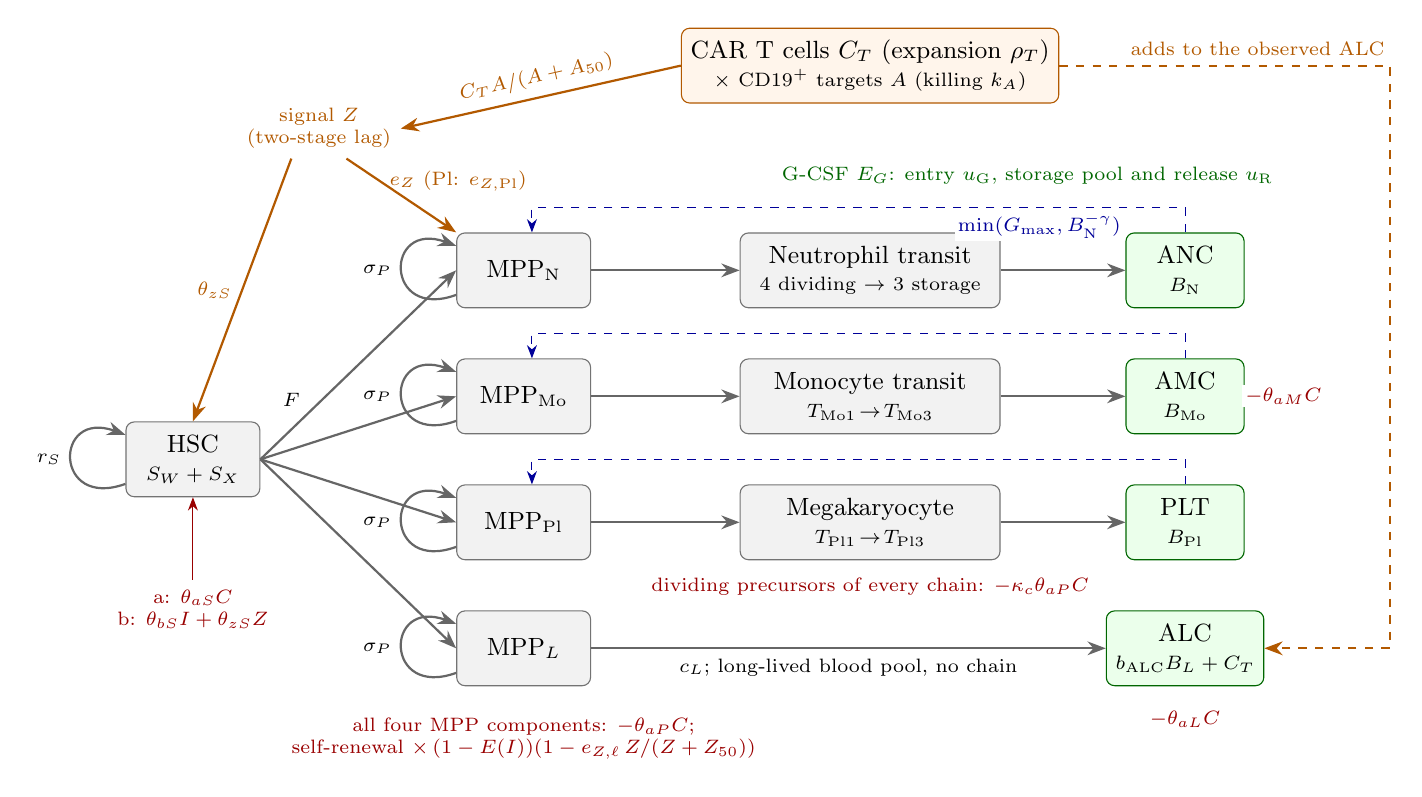
\begin{tikzpicture}[
  >=Stealth,
  box/.style={draw=black!55, rounded corners=3pt, fill=black!5, minimum height=0.95cm, minimum width=1.7cm, align=center, font=\small},
  blood/.style={box, fill=green!8, draw=green!40!black, minimum width=1.5cm},
  chain/.style={box, minimum width=3.3cm},
  arr/.style={->, thick, draw=black!60},
  sr/.style={->, thick, draw=black!60, looseness=5},
  fb/.style={->, dashed, draw=blue!60!black},
  inj/.style={->, draw=red!60!black},
  injl/.style={font=\scriptsize, text=red!60!black, align=center},
  zarr/.style={->, thick, draw=orange!70!black},
  zl/.style={font=\scriptsize, text=orange!70!black, align=center}]
\node[box] (HSC) at (0,0) {HSC\\[-1pt]\scriptsize $S_W+S_X$};
\node[box] (PN) at (4.2,2.4) {MPP$_{\mathrm{N}}$};
\node[box] (PM) at (4.2,0.8) {MPP$_{\mathrm{Mo}}$};
\node[box] (PP) at (4.2,-0.8) {MPP$_{\mathrm{Pl}}$};
\node[box] (PL) at (4.2,-2.4) {MPP$_{L}$};
\node[chain] (TN) at (8.6,2.4) {Neutrophil transit\\[-1pt]\scriptsize \valNkN{} dividing $\to$ \valNStore{} storage};
\node[chain] (TM) at (8.6,0.8) {Monocyte transit\\[-1pt]\scriptsize $T_{\mathrm{Mo}1}\!\to\!T_{\mathrm{Mo}3}$};
\node[chain] (TP) at (8.6,-0.8) {Megakaryocyte\\[-1pt]\scriptsize $T_{\mathrm{Pl}1}\!\to\!T_{\mathrm{Pl}3}$};
\node[blood] (ANC) at (12.6,2.4) {ANC\\[-1pt]\scriptsize $B_{\mathrm{N}}$};
\node[blood] (AMC) at (12.6,0.8) {AMC\\[-1pt]\scriptsize $B_{\mathrm{Mo}}$};
\node[blood] (PLT) at (12.6,-0.8) {PLT\\[-1pt]\scriptsize $B_{\mathrm{Pl}}$};
\node[blood] (ALC) at (12.6,-2.4) {ALC\\[-1pt]\scriptsize $b_{\mathrm{ALC}}B_L+C_T$};
\node[box, fill=orange!8, draw=orange!70!black, minimum width=4.2cm] (CART) at (8.6,5.0) {CAR T cells $C_T$ (expansion $\rho_T$)\\[-1pt]\scriptsize $\times$ CD19$^+$ targets $A$ (killing $k_A$)};
\node[zl] (Z) at (1.6,4.2) {signal $Z$\\(two-stage lag)};
\foreach \p in {PN,PM,PP,PL} \draw[arr] (HSC.east) -- (\p.west);
\node[font=\scriptsize] at (1.25,0.75) {$F$};
\draw[arr] (PN) -- (TN); \draw[arr] (PM) -- (TM); \draw[arr] (PP) -- (TP);
\draw[arr] (TN) -- (ANC); \draw[arr] (TM) -- (AMC); \draw[arr] (TP) -- (PLT);
\draw[arr] (PL) -- node[below, font=\scriptsize]{$c_L$; long-lived blood pool, no chain} (ALC);
\path (HSC) edge[sr, out=200, in=160, looseness=4] node[left, font=\scriptsize]{$r_S$} (HSC);
\foreach \p in {PN,PM,PP,PL} \path (\p) edge[sr, out=200, in=160, looseness=4] node[left, font=\scriptsize]{$\sigma_P$} (\p);
\foreach \b/\p in {ANC/PN,AMC/PM,PLT/PP} \draw[fb] (\b.north) -- ++(0,0.32) -| ([xshift=3pt]\p.north);
\node[font=\scriptsize, text=blue!60!black, fill=white, inner sep=1pt] at (10.75,2.97) {$\min(G_{\max},B_{\mathrm{N}}^{-\gamma})$};
\node[injl] (ia) at (0,-1.9) {a: $\theta_{aS}C$\\ b: $\theta_{bS}I+\theta_{zS}Z$};
\draw[inj] (ia) -- (HSC);
\node[injl] at (4.2,-3.55) {all four MPP components: $-\theta_{aP}C$;\\ self-renewal $\times\,(1-E(I))(1-e_{Z,\ell}\,Z/(Z+Z_{50}))$};
\node[injl] at (12.6,-3.3) {$-\theta_{aL}C$};
\node[injl, fill=white, inner sep=1pt] at (8.6,-1.62) {dividing precursors of every chain: $-\kappa_c\theta_{aP}C$};
\node[injl, fill=white, inner sep=1pt] at (13.85,0.8) {$-\theta_{aM}C$};
\draw[zarr] (CART.west) -- node[above, sloped, font=\scriptsize, text=orange!70!black]{$C_T A/(A+A_{50})$} (Z.east);
\draw[zarr] ([xshift=-0.35cm]Z.south) -- node[left, zl]{$\theta_{zS}$} (HSC.north);
\draw[zarr] ([xshift=0.35cm]Z.south) -- node[right, zl, pos=0.3]{$e_Z$ (Pl: $e_{Z,\mathrm{Pl}}$)} (PN.north west);
\draw[zarr, dashed] (CART.east) -- node[pos=0.6, above, zl]{adds to the observed ALC} (15.2,5.0) -- (15.2,-2.4) -- (ALC.east);
\node[font=\scriptsize, text=green!40!black, align=center] at (10.6,3.6) {G-CSF $E_G$: entry $u_{\mathrm{G}}$, storage pool and release $u_{\mathrm{R}}$};
\end{tikzpicture}}
\caption{Model3 (MarrowTwin). Loops mark self-renewal: $r_S$ for the HSC, the shared rate $\sigma_P$ for the four MPP components. Dashed blue: count feedback $\min(G_{\max},B_\ell^{-\gamma})$ on MPP self-renewal from the blood count of the same lineage (the lymphoid component has none). Red: injuries. Chemotherapy exposure $C$ injures the HSC ($\theta_{aS}$), all four MPP components ($\theta_{aP}$), the dividing precursors of every maturation chain ($\kappa_c\theta_{aP}$; in the neutrophil chain the first \valNkN{} of \valNTrN{} compartments, not the storage pool), circulating monocytes ($\theta_{aM}$) and blood lymphocytes ($\theta_{aL}$). In the CAR T phase, the lagged ferritin driver $I$ injures the HSC ($\theta_{bS}$) and, through $E(I)$, suppresses MPP self-renewal. Orange: the CAR T--target module; the interaction of CAR T cells with their targets produces the lagged signal $Z$, which injures the HSC ($\theta_{zS}$) and suppresses MPP self-renewal ($e_Z$; for the megakaryocyte component $e_{Z,\mathrm{Pl}}$, Model3 P2); CAR T cells add to the observed ALC. Green: G-CSF raises neutrophil chain entry and accelerates the transit through the storage pool into blood.}
\label{fig:model}
\end{figure}

% -----------------------------------------------------------------------------
\section{Inputs}
The inputs and their calibrations are those of Aim4 v1.3 (as in Model1 and Model2).

\subsection{Chemotherapy exposure (``a'')}
No drug concentrations are measured. A unitless exposure $C(t)$ summarises bridging and lymphodepleting chemotherapy:
\begin{align}
\frac{\dd C}{\dd t} &= u_a(t) - k_e C, \label{eq:C}\\
u_a(t) &= \lambda_{\mathrm{LD}}\left(\frac{90}{\mathrm{eGFR}}\right)^{\beta}\one[-5\le t<-2]
 \;+\; u_{\mathrm{br}}\,\one[t_{\mathrm{aph}}+\valBrFrom \le t < \valBrTo]. \label{eq:ua}
\end{align}
The first term is fludarabine--cyclophosphamide on days $-5$ to $-3$. It is scaled by renal function, because fludarabine is cleared by the kidney; eGFR is estimated with the race-free CKD-EPI 2021 equation from creatinine at lymphodepletion \citep{inker2021}. $\lambda_{\mathrm{LD}}$ is the dose fraction (1; 0.75 in the dose-reduction what-if). The second term is bridging chemotherapy, with rate $u_{\mathrm{br,RGO}}$ for R-GemOx and $u_{\mathrm{br,Cy}}$ for other regimens; it is zero without bridging chemotherapy. Bridging dates are not recorded, so the bridging window is assumed to run from two days after apheresis to day $-7$. $k_e$ is the elimination rate of the exposure.

\subsection{CAR T phase, ferritin route \texorpdfstring{(``b$_I$'')}{(b-I)}}
The ferritin driver $D(t)\geq 0$ is the patient's own inflammatory course, measured by ferritin $F$ relative to its value at lymphodepletion, $F_{\mathrm{LD}}$.
\begin{itemize}
\item \textbf{Fitting.} A cubic smoothing spline $\hat s(t)$ is fitted to $\log(F_i/F_{\mathrm{LD}})$ on days $\valFerFrom$ to $\valFerTo$, with degrees of freedom $\min(\max(4,\lfloor n/3\rfloor),8)$ for $n$ ferritin values ($n\geq4$; otherwise $D\equiv0$). Then $D(t)=0$ for $t<0$; $D(t)=\pos{\hat s(t)}$ up to the last ferritin day $t_F$; and after it $D(t)=\pos{\hat s(t_F)}\,e^{-\lambda_F(t-t_F)}$ with $\lambda_F=\valFerDecay$~d$^{-1}$. $D$ is stored on a \valDrvDt-day grid up to day \valDrvEnd{} and interpolated linearly.
\item \textbf{Prediction and simulation.} A gamma-shaped kernel is used:
\begin{equation}
D(t) = A_D\left(\frac{t}{t_p}\right)^{h}\exp\!\left[h\left(1-\frac{t}{t_p}\right)\right],\quad t>0;\qquad h=\valKernelH, \label{eq:kernel}
\end{equation}
with peak height $A_D$ on day $t_p$.
\end{itemize}
The driver reaches the marrow through a two-stage delay and acts there through a saturating effect:
\begin{align}
\frac{\dd I_1}{\dd t} &= k_I\,(D - I_1), \qquad \frac{\dd I}{\dd t} = k_I\,(I_1 - I), \label{eq:lag}\\
E(I) &= \frac{E_{\max} I^{h_E}}{I^{h_E} + \mathrm{IC}_{50}^{h_E}} \in [0, E_{\max}). \label{eq:E}
\end{align}
$I$ carries the irreversible HSC injury $\theta_{bS}$ (Eq.~\ref{eq:hsc}). $E(I)$ carries the reversible suppression of MPP self-renewal (Eq.~\ref{eq:G}); in Model3 (as in Model1 and Model2) this is its only site of action. $D$ itself does not act on the counts, because the screened platelet consumption term P1 is fixed at 0 (Section~\ref{sec:development}).

\subsection{CAR T phase, CAR T--target route \texorpdfstring{(``b$_Z$'')}{(b-Z)}}\label{sec:cart}
All patients in the extract received the same CD19-directed product (axicabtagene ciloleucel) after fludarabine--cyclophosphamide. CAR T cells in blood, $C_T$ ($10^9$/L, absolute), expand on CD19 antigen and contract; the antigen load $A$ (relative units; normal B cells and lymphoma together) is consumed by the CAR T cells; their interaction produces a signal that reaches the marrow through a two-stage lag:
\begin{align}
o(t) &= \frac{A}{A + A_{50}}, \label{eq:occ}\\
\frac{\dd C_T}{\dd t} &= \bigl(\rho_{T,i}\, o(t) - k_T\bigr)\, C_T, \label{eq:cart}\\
\frac{\dd A}{\dd t} &= -k_A\, C_T\, o(t), \label{eq:antigen}\\
\frac{\dd Z_1}{\dd t} &= k_Z\,\bigl(C_T\,o(t) - Z_1\bigr), \qquad \frac{\dd Z}{\dd t} = k_Z\,(Z_1 - Z). \label{eq:zlag}
\end{align}
\begin{itemize}
\item $o(t)$ is the antigen occupancy; $A_{50}$ is the antigen load at half-maximal occupancy.
\item $\rho_{T,i}$ is the patient's antigen-driven expansion rate (random effect) and $k_T$ the contraction rate.
\item $k_A$ is the rate at which CAR T cells clear their targets; the interaction term $C_T\,o(t)$ also drives the signal.
\item $Z$ is the lagged interaction signal (for example interferon-$\gamma$-type cytokines); $k_Z$ is the rate of each lag stage.
\item \textbf{Infusion.} $C_T=Z_1=Z=0$ before day 0. At day 0, $C_T(0^+)=C_T(0^-)+C_{T,0}$.
\item \textbf{Antigen load.} $A(t)=A_i(0)$ until the infusion, with $A_i(0)=\exp(\beta_A\,\mathrm{ldh}_{c,i})$ and $\mathrm{ldh}_{c,i}$ the patient's log LDH at lymphodepletion minus the cohort median; the median patient has $A(0)=1$.
\end{itemize}
$Z$ acts on the HSC as a second route of CAR T-phase injury ($\theta_{zS}$, Eq.~\ref{eq:hsc}) and on MPP self-renewal ($e_Z$, and $e_{Z,\mathrm{Pl}}$ for the megakaryocyte component; Eqs.~\ref{eq:G}--\ref{eq:ezpl}). The route variants of Section~\ref{sec:nested} switch one of the two effects off.

\subsection{G-CSF}\label{sec:gcsf}
G-CSF is given in windows $\mathcal W_i$; its effect $E_G\in[0,1)$ follows the dosing indicator,
\begin{equation}
\frac{\dd E_G}{\dd t} = k_G\,\bigl(\one[t\in\mathcal W_i] - E_G\bigr), \label{eq:gcsf}
\end{equation}
and acts on the neutrophil chain in two ways (Section~\ref{sec:chains}): entry is multiplied by $u_{\mathrm{N}}(t)=1+(u_{\mathrm{G}}-1)E_G(t)$, and the transit through the post-mitotic storage pool, including the release into blood, by $r_{\mathrm{N}}(t)=1+u_{\mathrm{R}}E_G(t)$. The storage-pool term produces the rapid ANC rise within a day of dosing; the entry term the slower increase of production. In Model2, whose storage pool was the single last compartment, $r_{\mathrm{N}}$ acted on the release from that compartment only.

\textbf{Imputed windows.} The extract records only whether G-CSF was needed after day 14, not dates or doses. The windows are therefore imputed by a fixed rule:
\begin{enumerate}
\item every patient: one dose on the day before each isolated ANC spike (Section~\ref{sec:obs}), window $[t_{\mathrm{spike}}-1,\,t_{\mathrm{spike}})$;
\item patients with G-CSF after day 14: a course of \valGcsfDays{} days from the first day $\geq\valGcsfFrom$ with an observed ANC $<\valGcsfThr$ (censored values count as low), repeated from the next such day after the end of a course, up to day \valGcsfUntil;
\end{enumerate}
overlapping windows are merged. Only ANC values that enter the likelihood are used. In the real cohort this gives \valGcsfWin{} windows in \valGcsfPts{} patients; \valGcsfNoWin{} of the \valGcsfFlagged{} flagged patients had no ANC $<\valGcsfThr$ after day \valGcsfFrom{} and receive no window. Landmark forecasts use only the windows up to the landmark (Section~\ref{sec:landmark}). TPO receptor agonists are used only in what-if analyses (entry factor $u_{\mathrm{T}}$ of the megakaryocyte chain while given).

% -----------------------------------------------------------------------------
\section{Haematopoietic model}\label{sec:haem}

\subsection{Stem cells with a pre-existing clone}
The HSC compartment contains normal ($S_W$) and clonal ($S_X$) cells that share one niche, $S=S_W+S_X$:
\begin{equation}
\frac{\dd S_j}{\dd t} = r_S\,S_j\,(1-S) - \left[\rho^a_j\,\theta_{aS}\,C + \rho^b_j\,\bigl(\theta_{bS}\,I+\theta_{zS}\,Z\bigr)\left(1+\eta\,\pos{1-S}\right)\right] S_j,\qquad j\in\{W,X\}.
\label{eq:hsc}
\end{equation}
\begin{itemize}
\item $r_S$ is the HSC self-renewal (regrowth) rate and measures marrow reserve; it is a random effect. Regrowth is limited by the niche: it is zero at the steady state $S=1$ and maximal when the pool is empty. Unlike Aim4, regrowth does not accelerate while the MPP is depleted (no $\alpha$; decision D1 of the Model1 plan).
\item $\theta_{aS}$ is the HSC injury rate per unit chemotherapy exposure. CAR T-phase injury has two routes: $\theta_{bS}$ per unit lagged ferritin driver (individual) and $\theta_{zS}$ per unit CAR T--target signal (population).
\item $\eta\geq0$ makes CAR T-phase injury stronger when the pool has already been depleted (synergy of ``a'' and ``b''; model Mab$\times$ only).
\item The relative sensitivities are $\rho^a_W=\rho^b_W=1$, $\rho^a_X=r_a$ and $\rho^b_X=r_b$.
\item Initial values are $S_W=1-f_0$ and $S_X=f_0$, with $f_0$ the pre-treatment clone fraction.
\end{itemize}
The stem cell output into the MPP components is
\begin{equation}
F = \frac{S_W + \delta\,S_X}{1-f_0+\delta f_0}, \label{eq:F}
\end{equation}
where $\delta$ is the output of a clonal relative to a normal HSC. The denominator makes $F=1$ at steady state for any $f_0$.

\subsection{MPP components}\label{sec:mpp}
The MPP layer has four components, one per blood lineage, $\ell\in\{\mathrm{N},\mathrm{Mo},\mathrm{Pl},L\}$. All four have the same form and the same rates:
\begin{equation}
\frac{\dd P_\ell}{\dd t} = (k_P-\sigma_P)\,F \;+\; \left(\sigma_P\,G_\ell - k_P\right) P_\ell \;-\; \theta_{aP}\,C\,P_\ell, \label{eq:mpp}
\end{equation}
\begin{equation}
G_\ell = \Phi_\ell\cdot\bigl(1-E(I)\bigr)\cdot\Bigl(1-e_{Z,\ell}\,\frac{Z}{Z+Z_{50}}\Bigr),\qquad
\Phi_\ell=\min\bigl(G_{\max},\,B_\ell^{-\gamma}\bigr)\ \ (\ell\in\{\mathrm{N},\mathrm{Mo},\mathrm{Pl}\}),\qquad \Phi_L=1, \label{eq:G}
\end{equation}
\begin{equation}
e_{Z,\mathrm{N}}=e_{Z,\mathrm{Mo}}=e_{Z,L}=e_Z,\qquad e_{Z,\mathrm{Pl}}=\logit^{-1}\bigl(\logit e_Z+d_{Z\mathrm{Pl}}\bigr). \label{eq:ezpl}
\end{equation}
\begin{itemize}
\item \textbf{Input from the stem cells:} $(k_P-\sigma_P)F$; all four components receive the same stem cell output.
\item \textbf{Exit rate $k_P$} (differentiation and death) and \textbf{self-renewal rate $\sigma_P<k_P$} at steady state. Both are shared by the four components and fixed at the Aim4 MPP values ($k_P=\valKp$, $\sigma_P=\valSrp$~d$^{-1}$; effective residence time $1/(k_P-\sigma_P)=\valResP$~d; Table~\ref{tab:selfrenewal}).
\item \textbf{Count feedback $\Phi_\ell$.} Each myeloid component senses only the blood count of its own lineage, $B_\ell$, as the proliferating compartment of \citet{friberg2002}. The exponent $\gamma$ is shared by the three myeloid components and estimated; the cap $G_{\max}$ is fixed. Lineages are therefore coupled only through the stem cell output and the shared inputs, and ANC and PLT can recover at different times.
\item \textbf{No feedback for lymphocytes} ($\Phi_L=1$). The Model1 plan had the same feedback for all four components. In the Model1 K1 a feedback on $P_L$ made the typical ALC overshoot to about 1.3 times baseline by day 30, because lymphodepletion keeps $B_L$ low for weeks while $P_L$ expands; it was therefore removed before any fit (Section~\ref{sec:deviations}).
\item \textbf{Suppression.} Marrow inflammation, $E(I)$, and the CAR T--target signal, $e_{Z,\ell}\,Z/(Z+Z_{50})$, reduce the self-renewal of all four components.
\item \textbf{Platelet-specific suppression by $Z$ (Model3 P2).} The megakaryocyte component has its own maximal suppression by the signal, $e_{Z,\mathrm{Pl}}$, a logit offset $d_{Z\mathrm{Pl}}$ from the shared $e_Z$ (Eq.~\ref{eq:ezpl}); $d_{Z\mathrm{Pl}}=0$ gives Model2. With $d_{Z\mathrm{Pl}}>0$ the CAR T--target interaction lowers platelet production more than the production of the other lineages, so that the late platelet fall can go with a strong CAR T expansion (Section~\ref{sec:why}). $d_{Z\mathrm{Pl}}$ is a population parameter, estimated on the identity scale with prior centre 0 and prior SD \valDzplSd. In models without the MPP route of $Z$ (suffix \texttt{\_Zh}) both $e_Z$ and $e_{Z,\mathrm{Pl}}$ are 0 and $d_{Z\mathrm{Pl}}$ is not estimated.
\item \textbf{Injury.} $\theta_{aP}$ is the individual MPP injury rate per unit chemotherapy exposure, the same for all four components.
\end{itemize}
Table~\ref{tab:selfrenewal} lists the self-renewing cells. Branch fractions and division amplification do not appear in Eq.~\ref{eq:mpp}: under normalisation they set only absolute compartment sizes and cancel.

\begin{table}[!htbp]
\centering
\footnotesize
\setlength{\tabcolsep}{3.5pt}
\caption{The self-renewing cells of Model3 (as Model1 and Model2). $k_P$: exit rate (differentiation and death, d$^{-1}$); $\sigma_P$: self-renewal rate at steady state (d$^{-1}$, $\sigma_P<k_P$); $\sigma_P/k_P$: share of a component's production that comes from self-renewal at steady state; $1/(k_P-\sigma_P)$: effective residence time (d). The four MPP components share $k_P$ and $\sigma_P$; the three myeloid components sense the blood count of their own lineage, the lymphoid component has no count feedback. All components' self-renewal is suppressed by marrow inflammation and by the CAR T--target signal; for the megakaryocyte component the maximal suppression by the signal is $e_{Z,\mathrm{Pl}}$ (Model3 P2).}
\label{tab:selfrenewal}
\begin{tabular}{lllllll>{\raggedright\arraybackslash}p{2.0cm}>{\raggedright\arraybackslash}p{1.9cm}}
\toprule
Cell & Self-renewal rate & $k_P$ & $\sigma_P$ & $\sigma_P/k_P$ & $1/(k_P-\sigma_P)$ & Count feedback & Suppressed by \\
\midrule
HSC & $r_S$ (random effect) & -- & 0.08 & -- & -- & niche $(1-S)$ & -- \\
MPP$_{\mathrm{N}}$ (neutrophils) & $\sigma_P$ (\texttt{sr\_p}) & 0.3 & 0.21 & 0.7 & 11.1 & $B_{\mathrm{N}}$ (ANC) & $E(I)$; $Z$ ($e_Z$) \\
MPP$_{\mathrm{Mo}}$ (monocytes) & $\sigma_P$ (\texttt{sr\_p}) & 0.3 & 0.21 & 0.7 & 11.1 & $B_{\mathrm{Mo}}$ (AMC) & $E(I)$; $Z$ ($e_Z$) \\
MPP$_{\mathrm{Pl}}$ (megakaryocytes) & $\sigma_P$ (\texttt{sr\_p}) & 0.3 & 0.21 & 0.7 & 11.1 & $B_{\mathrm{Pl}}$ (PLT) & $E(I)$; $Z$ ($e_{Z,\mathrm{Pl}}$) \\
MPP$_{L}$ (lymphocytes) & $\sigma_P$ (\texttt{sr\_p}) & 0.3 & 0.21 & 0.7 & 11.1 & none & $E(I)$; $Z$ ($e_Z$) \\
\bottomrule
\end{tabular}
\end{table}


\subsection{Maturation chains and blood}\label{sec:chains}
Each myeloid MPP component feeds a maturation chain and a blood compartment. The monocyte and megakaryocyte chains have three transit compartments, as in Model2, $\ell\in\{\mathrm{Mo},\mathrm{Pl}\}$:
\begin{align}
\frac{\dd T_{\ell1}}{\dd t} &= \kappa_\ell\left[P_\ell\,u_\ell(t) - T_{\ell1}\right] - \kappa_c\,\theta_{aP}\,C\,T_{\ell1}, \label{eq:chain1}\\
\frac{\dd T_{\ell2}}{\dd t} &= \kappa_\ell\left(T_{\ell1}-T_{\ell2}\right) - \kappa_c\,\theta_{aP}\,C\,T_{\ell2}, \qquad
\frac{\dd T_{\ell3}}{\dd t} = \kappa_\ell\left(T_{\ell2}-T_{\ell3}\right), \label{eq:chain2}\\
\frac{\dd B_\ell}{\dd t} &= c_\ell\left(T_{\ell3}-B_\ell\right) - \one[\ell=\mathrm{Mo}]\,\theta_{aM}\,C\,B_{\mathrm{Mo}}. \label{eq:blood}
\end{align}
The neutrophil chain (Model3 N) has $n_{\mathrm{N}}$ compartments; the first $k_{\mathrm{N}}$ are proliferating and the other $n_{\mathrm{N}}-k_{\mathrm{N}}$ form a post-mitotic storage pool:
\begin{align}
\frac{\dd T_{\mathrm{N}1}}{\dd t} &= \kappa_{\mathrm{N}}\left[P_{\mathrm{N}}\,u_{\mathrm{N}}(t) - T_{\mathrm{N}1}\right] - \kappa_c\,\theta_{aP}\,C\,T_{\mathrm{N}1}, \label{eq:nchain1}\\
\frac{\dd T_{\mathrm{N}j}}{\dd t} &= \kappa_{\mathrm{N}}\left(T_{\mathrm{N},j-1}-T_{\mathrm{N}j}\right) - \kappa_c\,\theta_{aP}\,C\,T_{\mathrm{N}j}, \qquad j=2,\dots,k_{\mathrm{N}}, \label{eq:nchain2}\\
\frac{\dd T_{\mathrm{N},k_{\mathrm{N}}+1}}{\dd t} &= \kappa_{\mathrm{N}}\left(T_{\mathrm{N}k_{\mathrm{N}}}-r_{\mathrm{N}}(t)\,T_{\mathrm{N},k_{\mathrm{N}}+1}\right), \label{eq:nchain3}\\
\frac{\dd T_{\mathrm{N}j}}{\dd t} &= \kappa_{\mathrm{N}}\,r_{\mathrm{N}}(t)\left(T_{\mathrm{N},j-1}-T_{\mathrm{N}j}\right), \qquad j=k_{\mathrm{N}}+2,\dots,n_{\mathrm{N}}, \label{eq:nchain4}\\
\frac{\dd B_{\mathrm{N}}}{\dd t} &= c_{\mathrm{N}}\left(r_{\mathrm{N}}(t)\,T_{\mathrm{N}n_{\mathrm{N}}}-B_{\mathrm{N}}\right), \label{eq:nblood}
\end{align}
with $n_{\mathrm{N}}=\valNTrN$ and $k_{\mathrm{N}}=\valNkN$ (design constants; Model2: $n_{\mathrm{N}}=\valNTrNModelTwo$, $k_{\mathrm{N}}=\valNkNModelTwo$, for which Eqs.~\ref{eq:nchain1}--\ref{eq:nblood} are the Model2 equations).
\begin{itemize}
\item \textbf{Transit rates.} $\kappa_{\mathrm{N}}=n_{\mathrm{N}}/\mathrm{MTT}_{\mathrm{N}}$ and $\kappa_\ell=3/\mathrm{MTT}_\ell$ for $\ell\in\{\mathrm{Mo},\mathrm{Pl}\}$, where $\mathrm{MTT}_\ell$ is the mean transit time through the whole chain; for megakaryocytes it is the maturation time, during which the cell undergoes endomitosis. At the prior centre $\mathrm{MTT}_{\mathrm{N}}=\valMttN$~d a neutrophil spends \valMttNProl~d in the proliferating part and \valMttNStore~d in the storage pool. With more compartments the transit time is less spread: its coefficient of variation is $1/\sqrt{n_{\mathrm{N}}}=0.38$, against $1/\sqrt3=0.58$ in Model2.
\item $c_\ell$ is the blood turnover rate.
\item \textbf{Kill of the proliferating precursors (Model2).} The proliferating compartments represent the dividing precursors: $T_{\mathrm{N}1}$ to $T_{\mathrm{N}k_{\mathrm{N}}}$ for neutrophils (myeloblasts to myelocytes), $T_{\ell1}$ and $T_{\ell2}$ for monocytes and megakaryocytes. Chemotherapy kills them at $\kappa_c\,\theta_{aP}\,C$, that is $\kappa_c$ times the patient's MPP kill rate. $\kappa_c$ is a population parameter, estimated with prior centre \valKappaC{} (as sensitive as the MPP) and prior SD \valKappaCSd{} on the log scale. $T_{\ell3}$ of the monocyte and megakaryocyte chains is not killed.
\item \textbf{Storage pool (Model3 N).} $T_{\mathrm{N},k_{\mathrm{N}}+1}$ to $T_{\mathrm{N}n_{\mathrm{N}}}$ represent the post-mitotic neutrophils of the marrow (metamyelocytes, band and segmented cells). Chemotherapy does not reach them, so after a hit the blood is supplied from the pool until it empties: compared with the Model2 chain at the same $\mathrm{MTT}_{\mathrm{N}}$, the ANC is held longer during lymphodepletion and then falls later and more steeply (Section~\ref{sec:kill}). G-CSF multiplies the transit rate of every storage compartment, including the release into blood, by $r_{\mathrm{N}}(t)$, and so mobilises the marrow reserve.
\item \textbf{Kill of circulating monocytes (Model2).} Blood monocytes are lost at $\theta_{aM}\,C$ in addition to their turnover; neutrophils and platelets in blood are not killed. $\theta_{aM}$ is a population parameter, estimated with the calibrated prior centre \valThAm{} (Section~\ref{sec:calibration}) and prior SD \valThAmSd{} on the log scale.
\item Apart from the kill terms the chains are delays: the count feedback and all suppression act in the MPP layer, as in the Friberg model. The production feedback at the chain entry ($B_\ell^{-\gamma_\ell}$) and the inflammation factor at the chain entry of Aim4 are not part of Model1, Model2 or Model3.
\item $u_\ell(t)$ is the effect of supportive care on entry: $u_{\mathrm{N}}=1+(u_{\mathrm{G}}-1)E_G$ (G-CSF, Eq.~\ref{eq:gcsf}), $u_{\mathrm{Pl}}=u_{\mathrm{T}}$ while a TPO receptor agonist is given (what-if only), and $u_{\mathrm{Mo}}=1$. $r_{\mathrm{N}}(t)=1+u_{\mathrm{R}}E_G$.
\item The engine also contains the screened term P1, $-\theta_{cP}\,D(t)\,B_{\mathrm{Pl}}$ in the platelet blood equation, with $\theta_{cP}$ fixed at \valThcp{} (Section~\ref{sec:development}); it has no effect.
\end{itemize}

\subsection{Lymphocytes}
The lymphoid component feeds a long-lived blood pool directly, without a maturation chain:
\begin{equation}
\frac{\dd B_L}{\dd t} = c_L\,(P_L-B_L) - \theta_{aL}\,C\,B_L. \label{eq:bl}
\end{equation}
$c_L$ is the turnover of blood lymphocytes and $\theta_{aL}$ the direct lymphodepletion. Both are calibrated (Section~\ref{sec:calibration}). CAR T cells are a separate compartment (Section~\ref{sec:cart}); they are added to $B_L$ only on the observed scale.

\subsection{Observed scale and interventions}
A model count is $Y_v(t)=b_{iv}\,B_v(t)$ for $v\in\{\mathrm{ANC},\mathrm{PLT},\mathrm{AMC}\}$, and
\begin{equation}
Y_{\mathrm{ALC}}(t)=b_{i,\mathrm{ALC}}\,B_L(t)+C_T(t), \label{eq:alc}
\end{equation}
where $b_{iv}$ is the patient's set point, an individual parameter (Section~\ref{sec:baseline}). A CD34$^+$ boost of size $\Delta S$ on day $t_c$ sets $S_W(t_c^+)=S_W(t_c^-)+\Delta S$.

\subsection{Steady state, nesting, Friberg limit and one-way coupling}\label{sec:steady}
\textbf{Steady state.} With $C=I_1=I=D=0$, $C_T=Z_1=Z=E_G=0$ and $A=A_i(0)$, the state ``all haematopoietic compartments $=1$, $S_W=1-f_0$, $S_X=f_0$'' is a steady state: $1-S=0$ and $F=1$; every $B_\ell=1$, so $G_\ell=1$ and Eq.~\ref{eq:mpp} gives $(k_P-\sigma_P)+(\sigma_P-k_P)=0$; the chains and blood are linear relaxations onto their inputs ($r_{\mathrm{N}}=1$ without G-CSF); without CAR T cells the antigen load does not change. The directions $S_X/S$ and $A$ are neutral. The engine reserves \valNTnSlots{} neutrophil compartments; with $n_{\mathrm{N}}=\valNTrN$ the unused one stays constant.

\textbf{Nesting of Model2 and Model1.} With $n_{\mathrm{N}}=\valNTrNModelTwo$, $k_{\mathrm{N}}=\valNkNModelTwo$ and $d_{Z\mathrm{Pl}}=0$ (and $\theta_{cP}=0$) the equations of Model3 are those of Model2; with $\kappa_c=\theta_{aM}=0$ in addition, those of Model1. The K1 unit tests compare Model3 with these values against frozen copies of the Model2 v1.0 engine (models Mab, MabC\_ddr, Mab$\times$\_Zm and Mb) and of the Model1 v1.0 engine (Mab, MabC\_ddr and Mab$\times$\_Zm), with the CAR T infusion and a ferritin driver: all outputs agree within $10^{-6}$. (The constant unused compartments enter the step-size control of the integrator, so the agreement is not to machine precision.) The drop-one models \texttt{\_noN} and \texttt{\_noP2} carry exactly these values (Section~\ref{sec:nested}). The kill terms are zero without chemotherapy, P2 is zero without CAR T--target signal, and N does not change the steady state; so none of them changes the calibrations of the CAR T module. N changes the stability of the steady state (below).

\textbf{Friberg limit.} If $\sigma_P\to k_P$, the stem cell input vanishes and Eq.~\ref{eq:mpp} becomes
\begin{equation*}
\frac{\dd P_\ell}{\dd t} = k_P\,P_\ell\,\bigl(\Phi_\ell-1\bigr) - \theta_{aP}\,C\,P_\ell
\end{equation*}
(without inflammation and $Z$, and with $\kappa_c=\theta_{aM}=0$): the proliferating compartment of \citet{friberg2002} with $k_{\mathrm{prol}}=k_P$, the feedback $\min(G_{\max},B_\ell^{-\gamma})$, and the drug effect as a kill term rather than a factor $(1-E)$ on proliferation. Model1, Model2 and Model3 are thus Friberg-type chains with a stem cell layer on top. The unit tests compare this limit, with the three-compartment chain of Model2, with an independent deSolve implementation (Section~\ref{sec:calibration}).

\textbf{One-way lymphoid branch.} No equation of the myeloid lineages, the stem cells, the CAR T--target module or the inputs contains $P_L$ or $B_L$. The fitted ANC, PLT and AMC are therefore independent of $c_L$ and $\theta_{aL}$.

\textbf{Changes that act on one lineage.} $\theta_{aM}$ appears only in the equation of $B_{\mathrm{Mo}}$, the neutrophil chain constants $n_{\mathrm{N}}$ and $k_{\mathrm{N}}$ only in the neutrophil chain, and $d_{Z\mathrm{Pl}}$ only in the megakaryocyte MPP component, where it acts only through $Z$. Through the count feedback each also changes the MPP component of its own lineage, but no other lineage, the stem cells or ALC (K1: other outputs unchanged within $10^{-6}$). The CAR T--target module acts on ANC, PLT and AMC through $Z$ and is informed by ALC through $C_T$ (Eq.~\ref{eq:alc}).

\textbf{Stability.} The stem cell output does not depend on the blood counts, so at the steady state the lineages are decoupled, and each is stable or unstable on its own. A longer delay in a count feedback loop destabilises it. At $\sigma_P=\valSrp$ the steady state loses stability (Hopf bifurcation) at $\gamma=\valHopf$ with the Model3 neutrophil chain and $\mathrm{MTT}_{\mathrm{N}}=\valMttN$~d; with the Model2 chain it is $\gamma=\valHopfModelTwoChain$, a value set by the \valHopfOtherLineage{} lineage. The Hopf point falls as $\mathrm{MTT}_{\mathrm{N}}$ grows, to $\gamma=\valHopfMttHi$ at $\mathrm{MTT}_{\mathrm{N}}=\valMttNHi$~d (Model2 chain: \valHopfMttHiModelTwo; Table~\ref{tab:hopf}). The search box is therefore limited to $\gamma\leq\valGammaHi$ and $\mathrm{MTT}_{\mathrm{N}}\leq\valMttNHi$~d (Model2: $\gamma\leq\valGammaHiModelTwo$), so that every point of it is stable: on a grid over the search boxes of the three maturation times at $\gamma=\valGammaHi$ the largest real part of the eigenvalues is $\valBoxMaxRe$~d$^{-1}$. Near this corner, oscillations are damped only slowly. Table~\ref{tab:stability} shows the stability over $\gamma$ and $\sigma_P$ at the prior centres; with $\sigma_P$ scaled by 1.2 stability is lost from $\gamma\approx1.5$; $\sigma_P$ is fixed in the fits.

\begin{table}[!htbp]
\centering
\small
\setlength{\tabcolsep}{3.5pt}
\caption{Value of $\gamma$ at which the pre-treatment steady state loses stability (Hopf bifurcation), at $\sigma_P=0.21$ and the prior centres otherwise, as a function of $\mathrm{MTT}_{\mathrm{N}}$ (from the lower to the upper limit of its search box), for the Model3 neutrophil chain ($n_{\mathrm{N}}=7$, $k_{\mathrm{N}}=4$) and the Model2 chain (3 and 2). 2.37 is the value set by the megakaryocyte lineage, which applies when the neutrophil lineage is more stable. The search box of $\gamma$ ends at 1. On a $6\times6\times6$ grid over the search boxes of $\mathrm{MTT}_{\mathrm{N}}$, $\mathrm{MTT}_{\mathrm{Pl}}$ and $\mathrm{MTT}_{\mathrm{Mo}}$ at $\gamma=1$, the largest real part of the eigenvalues is $-0.004$~d$^{-1}$.}
\label{tab:hopf}
\begin{tabular}{rrr}
\toprule
$\mathrm{MTT}_{\mathrm{N}}$ (d) & Hopf $\gamma$, Model3 chain & Hopf $\gamma$, Model2 chain \\
\midrule
0.677 & 2.37 & 2.37 \\
2 & 2.37 & 2.37 \\
3.5 & 2.37 & 2.37 \\
5 & 2.09 & 2.37 \\
8.5 & 1.48 & 2.25 \\
12 & 1.22 & 1.95 \\
15 & 1.10 & 1.82 \\
\bottomrule
\end{tabular}
\end{table}


\subsection{Effect of the kill terms and the storage pool on the typical patient}\label{sec:kill}
In the typical design without CAR T phase and without HSC injury (Table~\ref{tab:aim4}):
\begin{itemize}
\item $\kappa_c$ deepens the nadir of every lineage (K1 test: the minimum of ANC, PLT and AMC from day 0 is lower with $\kappa_c=1$ than with $\kappa_c=0$); with the Model2 values the typical ANC nadir is \valAncNadirModelTwo{} times baseline on day \valAncNadirDayModelTwo{} (Model1 values: \valAncNadirModelOne{} on day \valAncNadirDayModelOne).
\item \textbf{Storage pool.} At the same $\mathrm{MTT}_{\mathrm{N}}$ (\valMttN~d), the Model3 chain holds the typical ANC higher during lymphodepletion (mean \valAncPreModel{} times baseline on days $-5$ to $-1$; Model2 chain \valAncPreModelTwo; observed median 0.83, Section~\ref{sec:why}) and lower afterwards (days 5--9: \valAncMidModel; Model2 chain \valAncMidModelTwo; observed 0.06). The typical nadir is \valAncNadirModel{} times baseline on day \valAncNadirDayModel. It is deeper than with the Model2 chain but, at the prior centres, still earlier than observed (day 7); in the N screen the data moved $\mathrm{MTT}_{\mathrm{N}}$ to \valNScreenMtt~d (Table~\ref{tab:nscreen}). $\kappa_c$ and the maturation times are left to the data. Killing more compartments of the same chain deepens the nadir (K1 test).
\item The typical AMC on days $-1$ to 0 equals the observed median (\valAmcTarget) by the calibration of $\theta_{aM}$; its nadir is \valAmcNadirModel{} times baseline on day \valAmcNadirDayModel. N and P2 do not change PLT, AMC or ALC in this design.
\end{itemize}

\subsection{Reachable phenotypes}\label{sec:reachable}
The count feedback lets an MPP component sustain itself without stem cell output. Without suppression and with $F\approx0$, the quasi-steady level of a myeloid component solves $\sigma_P\,\Phi_\ell(P^\ast)=k_P$ with $B_\ell\approx P^\ast$, that is $P^\ast=(k_P/\sigma_P)^{-1/\gamma}=\valPstar$ at the prior centre of $\gamma$. A screen in K1 (Table~\ref{tab:screen}) gives the following structural property, as in Model1 and Model2:
\begin{itemize}
\item \textbf{A chemotherapy hit alone gives quick or delayed recovery, never a second wave.} In the Model3 screen a single hit by bridging and lymphodepleting chemotherapy gave quick recovery for most screened reserves and HSC injuries and delayed recovery for the strongest injury ($\theta_{aS}=2.5$) with low reserve ($r_S\leq0.04$); with the Model2 chain the whole grid gave quick recovery. In the unit test a deeper hit ($\theta_{aS}=3$, $r_S=0.03$) gave delayed recovery, and no hit gave a second wave. In Model1 the same held for $\gamma$ from 0.5 to 3, and with the CAR T phase present but without CAR T-phase HSC injury. Aim4 could produce a ``pseudo second wave'' from one hit, through the oscillation of its several self-renewing progenitor layers; Model1, Model2 and Model3 did not in any screened setting.
\item \textbf{A second wave needs the CAR T phase.} It arises when CAR T-phase HSC injury ($\theta_{bS}$ or $\theta_{zS}$) coincides with suppression of MPP self-renewal by $E(I)$ and $Z$; in the screen this required $E_{\max}\geq0.5$, a strong driver and $\theta_{bS}>0$.
\end{itemize}
In M0 and Ma, which have no CAR T-phase HSC injury, a second wave is therefore almost unreachable. The comparison of the Q2 models is partly determined by this structure. The synthetic design S4 (Section~\ref{sec:validation}), in which the data are generated by the Aim4 engine and fitted with Model3, quantifies the consequence for the ``when'' readout.

\begin{table}[!htbp]
\centering
\small
\setlength{\tabcolsep}{3.5pt}
\caption{Phenotypes that the CAR T phase alone can give (model Mb, typical design, ANC set point 3.5, prior centres otherwise) over the driver peak $A_D$ (peak day 9), the ferritin-route HSC injury $\theta_{bS}$ and $E_{\max}$. Q: quick; SW: second wave; D: delayed. A chemotherapy hit alone (model Ma, no CAR T phase; $r_S\in\{0.02,0.04,0.08\}$, $\theta_{aS}\in\{0.4,1,1.5,2.5\}$) gave only delayed or quick recovery.}
\label{tab:screen}
\begin{tabular}{rrcccc}
\toprule
$A_D$ & $\theta_{bS}$ & $E_{\max}=0.3$ & $E_{\max}=0.5$ & $E_{\max}=0.7$ & $E_{\max}=0.9$ \\
\midrule
1 & 0 & Q & Q & Q & Q \\
1 & 0.02 & Q & Q & Q & Q \\
1 & 0.06 & Q & Q & Q & Q \\
1.5 & 0 & Q & Q & Q & Q \\
1.5 & 0.02 & Q & Q & Q & Q \\
1.5 & 0.06 & Q & Q & Q & Q \\
2.5 & 0 & Q & Q & Q & Q \\
2.5 & 0.02 & Q & Q & Q & Q \\
2.5 & 0.06 & Q & Q & SW & SW \\
3.5 & 0 & Q & Q & Q & Q \\
3.5 & 0.02 & Q & Q & Q & SW \\
3.5 & 0.06 & Q & SW & SW & SW \\
\bottomrule
\end{tabular}
\end{table}


% -----------------------------------------------------------------------------
\section{Reference model MF}\label{sec:mf}
MF is the original Friberg model \citep{friberg2002}, with one independent chain per lineage $\ell\in\{\mathrm{N},\mathrm{Pl},\mathrm{Mo}\}$:
\begin{align}
\frac{\dd \mathrm{Prol}_\ell}{\dd t} &= k_\ell\,\mathrm{Prol}_\ell\,(1-E_\ell)\,B_\ell^{-\gamma^{\mathrm{MF}}} - k_\ell\,\mathrm{Prol}_\ell,\qquad
\frac{\dd T_{\ell j}}{\dd t} = k_\ell(T_{\ell,j-1}-T_{\ell j}),\qquad
\frac{\dd B_\ell}{\dd t} = k_\ell(T_{\ell3}-B_\ell),
\end{align}
\begin{itemize}
\item $k_{\mathrm{prol}}=k_{\mathrm{tr}}=k_{\mathrm{circ}}=k_\ell=4/(\mathrm{MTT}^{\mathrm{MF}}_\ell\,s_{\mathrm{MTT},i})$;
\item drug effect $E_{\mathrm{N}}=\mathrm{Slope}_i\,C$ and $E_\ell=\rho_\ell\,\mathrm{Slope}_i\,C$ for the other lineages;
\item the exposure $C$ is the same as in Eq.~\ref{eq:C};
\item there is no stem cell layer, no CAR T-phase input, no CAR T compartment, no G-CSF effect, no kill of chain precursors or blood monocytes, no storage pool, and no ALC;
\item two random effects, $\mathrm{Slope}$ and $s_{\mathrm{MTT}}$ (Table~\ref{tab:re}), and individual baselines for ANC, PLT and AMC; population parameters in Table~\ref{tab:mf}.
\end{itemize}
MF serves as the benchmark in the model comparison, on the ANC, PLT and AMC part of the likelihood with the same phenotype term (Section~\ref{sec:pheno}). MF is not refitted for Model3: its engine, data and phenotype term are those of Model2, and the converged Model2 fit of MF is reused (pre-registered deviation, Section~\ref{sec:deviations}).

% -----------------------------------------------------------------------------
\section{Data and observation model}\label{sec:obs}

\subsection{Data handling}
Daily ANC, PLT, AMC and ALC ($\times10^9$/L) come from the de-identified extract (35 patients). The source file is read-only, and its SHA-256 is checked at every conversion. The following rules apply:
\begin{enumerate}
\item \textbf{Blank differential.} If the differential is blank and WBC $<\valWbcNoDiff$, ANC, AMC and ALC are left-censored at WBC.
\item \textbf{Zero on a manual differential.} The value is left-censored at WBC$/\valManualCells$.
\item \textbf{G-CSF.} An isolated G-CSF spike is a value $\geq1.5$ that is at least twice the previous value, with the previous and the next value $<1.0$. Spikes anchor the imputed G-CSF windows (Section~\ref{sec:gcsf}); ANC values under G-CSF, spikes included, are ordinary observations.
\item \textbf{Platelet transfusion.} Platelet type is not recorded, so a transfusion is inferred when PLT $<\valPltBelow$ on a transfusion day, or when PLT rises by more than \valPltRise{} on the next day without a haemoglobin rise above \valHgbRise. The next \valPltDrop{} days of PLT are excluded.
\item \textbf{Follow-up.} Values after progression or after day \valObsMax{} are excluded.
\item \textbf{Set points.} The set point median $m_{iv}$ is the median of the uncensored values on days $\valSetFrom$ to $\valSetTo$ (with bridging chemotherapy: up to the apheresis day). The rows that define it enter the fit only through the baseline prior (Section~\ref{sec:baseline}).
\item \textbf{Covariates of the CAR T module.} LDH at lymphodepletion (all 35 patients) sets the initial antigen load. The measured peak CAR T expansion is available for 16 patients, without recorded units; it is not fitted and serves only as an external check (test T8).
\end{enumerate}

\subsection{Individual baselines}\label{sec:baseline}
Each patient has one baseline per lineage $v\in\{\mathrm{ANC},\mathrm{PLT},\mathrm{AMC},\mathrm{ALC}\}$ (MF: the first three),
\begin{equation}
\log b_{iv} = \log m_{iv} + d_{iv},\qquad d_{iv}\sim N\Bigl(0,\ \frac{s_v^2}{n_{iv}}+\tau_v^2\Bigr), \label{eq:baseprior}
\end{equation}
where $n_{iv}$ is the number of set-point values of patient $i$, $s_v$ the pooled within-patient SD of the log set-point values (fixed from the data) and $\tau_v$ the set-point drift (population parameter, estimated). Table~\ref{tab:baseline} gives $s_v$ and $n_{iv}$.

\begin{table}[!htbp]
\centering
\small
\setlength{\tabcolsep}{3.5pt}
\caption{Individual baselines. $s_v$: pooled within-patient SD of the log set-point values (data, fixed); $n_{iv}$: number of set-point values of a patient (median, range); these rows enter only through the prior. The set-point drift $\tau_v$ starts at 0.3, is shrunk with $\nu=4$ towards it and is bounded below by 0.02.}
\label{tab:baseline}
\begin{tabular}{lrrr}
\toprule
Lineage & $s_v$ & $n_{iv}$ & Set-point rows \\
\midrule
ANC & 0.352 & 4 (1--8) & 145 \\
PLT & 0.184 & 4 (1--8) & 151 \\
AMC & 0.46 & 4 (1--8) & 145 \\
ALC & 0.321 & 4 (1--8) & 145 \\
\bottomrule
\end{tabular}
\end{table}


\subsection{Likelihood of the counts}
For $v\in\{\mathrm{ANC},\mathrm{PLT},\mathrm{AMC},\mathrm{ALC}\}$, an observation $y$ on day $t$ has
\begin{equation}
\log y = \log Y_v(t;\psi_i) + \epsilon,\qquad \epsilon\sim N(0,\sigma_v^2). \label{eq:obs}
\end{equation}
A left-censored value contributes $\Phi\bigl((\log y-\log Y_v(t))/\sigma_v\bigr)$. The ANC, PLT and AMC part is also computed on its own, for the comparison with MF. In simulation designs with measured variant allele fractions, a positive clone fraction $f_{\mathrm{obs}}$ adds $\log N(\log f_{\mathrm{obs}};\log f_0,s^2)$ and a negative result at detection limit $\ell_d$ adds $\log\Phi((\log 2\ell_d-\log f_0)/s)$.

\subsection{Recovery phenotypes}\label{sec:phenotypes}
The same rule \citep[thresholds of][]{rejeski2021} classifies observed series and model trajectories:
\begin{enumerate}
\item Use ANC on days 0 to \valPhWin. Set left-censored values to \valCensVal{} and remove isolated G-CSF spikes.
\item The nadir is the minimum on days \valNadFrom--\valNadTo.
\item Recovery is the first value $\geq\valRec$ after the nadir. Without recovery the class is \emph{delayed}.
\item A value $<\valDip$ after recovery makes the class \emph{second wave}; otherwise it is \emph{quick}.
\end{enumerate}
In the real cohort the rule gives \valNQuick{} quick, \valNSecond{} second-wave and \valNDelayed{} delayed patients. In simulations with follow-up to day 75, \emph{persistent} (a median ANC on days \valPersFrom--\valPersTo{} below \valPersThr) is assessed first. Five pre-specified variants serve as sensitivity analyses: window to day 35; second-wave dip counted only after day 21; two consecutive values required for recovery and for the dip; recovery threshold 1.0; dip threshold 0.5.

\subsection{Phenotype term}\label{sec:pheno}
The observed phenotype $c_i$ of patient $i$ (primary rule) enters the likelihood through the model probability of that class. The probability is computed from the model ANC $\mu(t)=b_{i,\mathrm{ANC}}B_{\mathrm{N}}(t)$ on the patient's \emph{label days}: the days the rule used for the observed label (days 0--\valPhWin, isolated G-CSF spikes removed). On the log scale, with $x(t)=\log\mu(t)$:
\begin{enumerate}
\item \textbf{Nadir.} $j^\ast$ is the label day with the smallest $x$ on days \valNadFrom--\valNadTo.
\item \textbf{Recovery margin.} $m_R=\max_{t>j^\ast}\,\bigl[x(t)-\log\valRec\bigr]$, the largest excess over the recovery threshold after the nadir (for a rule with $n$ consecutive values: the minimum of $n$ consecutive values).
\item \textbf{Recovery day.} $r^\ast$ is the first label day after $j^\ast$ with a positive recovery margin; if there is none, the day with the largest margin. In this way $r^\ast$ moves continuously when the model ANC just reaches the threshold.
\item \textbf{Dip margin.} $m_D=\max_{t>r^\ast}\,\bigl[\log\valDip-x(t)\bigr]$, over days at or after the dip start of the rule (for $n$ consecutive values: the maximum of $n$ consecutive values).
\item \textbf{Soft classification} with smoothing scale $s$:
\begin{equation}
\begin{aligned}
P(\mathrm{delayed}) &= 1-\Phi\!\Bigl(\frac{m_R}{s}\Bigr),\\
P(\mathrm{second\ wave}) &= \Phi\!\Bigl(\frac{m_R}{s}\Bigr)\,\Phi\!\Bigl(\frac{m_D}{s}\Bigr),\\
P(\mathrm{quick}) &= \Phi\!\Bigl(\frac{m_R}{s}\Bigr)\Bigl[1-\Phi\!\Bigl(\frac{m_D}{s}\Bigr)\Bigr].
\end{aligned} \label{eq:psoft}
\end{equation}
\item \textbf{Label error.} $P'(c)=(1-3\varepsilon)\,P(c)+\varepsilon$.
\end{enumerate}
The term added to the log-likelihood of patient $i$ is $w\log P'(c_i\mid\psi_i)$, with $w=\valPhW$, $s=\valPhS$ and $\varepsilon=\valPhEps$.
\begin{itemize}
\item As $s\to0$ the classification equals the rule applied to the model series on the label days (checked in K1). With $s=\valPhS$, a model maximum of 2.0 after the nadir (that is, $1.5e^{0.3}$) gives $P(\text{recovered})=\Phi(1)=0.84$.
\item $\varepsilon$ bounds the term of one patient by $-w\log\varepsilon=\valPhFloor$, so a single patient cannot dominate the fit.
\item The term uses only existing model output; it adds no state.
\item \textbf{Composite likelihood.} The phenotype is a function of the same day 0--\valPhWin{} ANC values that enter Eq.~\ref{eq:obs}. Adding the term uses these data twice. The objective is therefore a composite (weighted) likelihood, not the likelihood of a probability model; $w$ sets the weight, and $w=0$ gives the count likelihood alone. Posterior intervals are expected to be too narrow. BIC values are compared only between models with the same term; MF receives the same term, computed from its ANC.
\item The term is not used at landmarks (Section~\ref{sec:landmark}), because the phenotype is the quantity that is predicted there.
\end{itemize}
Sensitivity analyses: $s=\valPhSensS$, and $w=\valPhSensW$.

% -----------------------------------------------------------------------------
\section{Statistical model and estimation}\label{sec:stat}

\subsection{Individual parameters}
Each patient has up to six random effects $\psi_{ik}=g_k^{-1}(\eta_{ik})$, with
\begin{equation}
\eta_{ik} = \mu_k + \boldsymbol\beta_k^\top \mathbf{x}_{ik} + \omega_k z_{ik},\qquad z_{ik}\sim N(0,1),
\end{equation}
and the baseline deviations $d_{iv}$ of Eq.~\ref{eq:baseprior}; together they form the individual vector $\psi_i$ (ten components in the largest model). The link $g_k$ is the log for rates and the logit for $f_0$. The covariates $\mathbf{x}$ are listed in Table~\ref{tab:re}. Each patient's parameters are restricted to a physiological box (Table~\ref{tab:box}), which acts as the support of a truncated prior.

All other parameters are population parameters (Tables~\ref{tab:struct_marrow}--\ref{tab:struct_cart}). Of these, the following are estimated:
\begin{itemize}
\item in every Model3 model: $\mathrm{MTT}_{\mathrm{N}}$, $\mathrm{MTT}_{\mathrm{Pl}}$, $\mathrm{MTT}_{\mathrm{Mo}}$, $\mathrm{IC}_{50}$, $k_I$, $\gamma$, $u_{\mathrm{br,RGO}}$, $E_{\max}$, $k_T$, $\beta_A$, $u_{\mathrm{G}}$, $u_{\mathrm{R}}$ (as Model1; Aim4: $\gamma_M$ in place of $\gamma$ and $e_{\mathrm{sr}}$ in place of $E_{\max}$), and the two kill parameters $\kappa_c$ and $\theta_{aM}$ (Model2);
\item $\theta_{zS}$ in the models with CAR T-phase HSC injury (Mb, Mab, Mab$\times$) unless the HSC route is switched off; $e_Z$ and $d_{Z\mathrm{Pl}}$ (new in Model3) in every model unless the MPP route is switched off;
\item $\eta$ in Mab$\times$.
\end{itemize}
Each has a normal prior on the working scale (log; logit for $E_{\max}$ and $e_Z$; identity for $d_{Z\mathrm{Pl}}$) centred at its default: SD \valStructSd{} in general; SD \valEmaxSd{} for $\logit E_{\max}$, SD \valThzsSd{} for $\log\theta_{zS}$, SD \valEzSd{} for $\logit e_Z$, SD \valKappaCSd{} for $\log\kappa_c$, SD \valThAmSd{} for $\log\theta_{aM}$ and SD \valDzplSd{} for $d_{Z\mathrm{Pl}}$ (centre 0, so that a priori $e_{Z,\mathrm{Pl}}=e_Z$); $\log\eta\sim N(\valEtaCentre,\valEtaSd^2)$. The search box is the prior centre $\pm4$ prior SD on the working scale, with $u_{\mathrm{G}}\in[\valGcsfFoldLo,\valGcsfFoldHi]$, $\gamma\leq\valGammaHi$ and $\mathrm{MTT}_{\mathrm{N}}\leq\valMttNHi$~d (Section~\ref{sec:steady}). This gives $\gamma\in[\valGammaLo,\valGammaHi]$, $\mathrm{MTT}_{\mathrm{N}}\in[\valMttNLo,\valMttNHi]$~d and $d_{Z\mathrm{Pl}}\in[\valDzplLo,\valDzplHi]$, that is $e_{Z,\mathrm{Pl}}\in[\valEzPlLo,\valEzPlHi]$ with $e_Z$ at its centre; in the P2 screen $d_{Z\mathrm{Pl}}$ went beyond this box (Section~\ref{sec:development}), and an estimate on a bound is reported. The remaining parameters are fixed, among them $\theta_{cP}=\valThcp$; $n_{\mathrm{N}}$ and $k_{\mathrm{N}}$ are design constants and are not estimated.

\begin{table}[!htbp]
\centering
\footnotesize
\setlength{\tabcolsep}{3.5pt}
\caption{Individual parameters (random effects). $\psi_{ik}=g_k^{-1}(\eta_{ik})$ with $\eta_{ik}=\mu_k+\boldsymbol\beta_k^\top\mathbf{x}_{ik}+\omega_k z_{ik}$, $z_{ik}\sim N(0,1)$. Centre: the prior centre $g_k^{-1}(\mu_k)$ (the Model3 wave-1 fits start from the Model2 population instead, Section~\ref{sec:nested}); $\omega_k$: prior spread on the working scale (the estimate is shrunk towards it, Section~\ref{sec:its}). The $\theta_{aP}$ centre is kept from Model1 and the $\rho_T$ centre is calibrated (Section~\ref{sec:calibration}). Each patient also has one baseline deviation per lineage (Section~\ref{sec:baseline}).}
\label{tab:re}
\begin{tabular}{ll>{\raggedright\arraybackslash}p{5.4cm}lll>{\raggedright\arraybackslash}p{3.2cm}}
\toprule
Symbol & Code & Meaning & Scale $g_k$ & Centre & $\omega_k$ & Covariates $\mathbf{x}$ \\
\midrule
$r_S$ & \texttt{r\_s} & HSC self-renewal (regrowth) rate; reserve, Q1 & log & 0.08 & 0.5 & prior lines, prior ASCT, age \\
$f_0$ & \texttt{f0} & Pre-treatment clone fraction of the HSC pool, Q1 & logit & 0.02 & 1.5 & age, prior lines, prior ASCT, log RDW, MCV \\
$\theta_{aS}$ & \texttt{th\_as} & HSC injury per unit chemotherapy exposure (a), Q2 & log & 0.12 & 0.8 & -- \\
$\theta_{aP}$ & \texttt{th\_ap} & MPP injury per unit exposure (all four components; proliferating chain precursors at $\kappa_c\theta_{aP}$) & log & 2.71 & 0.5 & -- \\
$\theta_{bS}$ & \texttt{th\_bs} & HSC injury per unit lagged ferritin driver (ferritin route of b), Q2 & log & 0.02 & 1 & -- \\
$\rho_T$ & \texttt{rho} & CAR T antigen-driven expansion rate (all Model3 models) & log & 0.811 & 0.5 & -- \\
$\mathrm{Slope}$ & \texttt{slope} & MF: drug effect per unit exposure & log & 1.5 & 0.5 & -- \\
$s_{\mathrm{MTT}}$ & \texttt{mtt\_scale} & MF: individual scaling of all MTTs & log & 1 & 0.2 & -- \\
\bottomrule
\end{tabular}
\end{table}

\begin{table}[!htbp]
\centering
\small
\setlength{\tabcolsep}{3.5pt}
\caption{Search box of the individual parameters (natural scale). The box is the support of each patient's parameters: the prior is truncated to it, the differential-evolution search, the importance sampling and the MCMC stay inside it, and fitted values on a bound are reported. Round 0 (used only by fits that do not start from another fit) widens the prior but keeps this box. Baseline deviations $d_{iv}$ have the box $\pm\max(1,\ 4\,s_{iv})$, with $s_{iv}$ the prior SD of Eq.~\ref{eq:baseprior}.}
\label{tab:box}
\begin{tabular}{llrrr}
\toprule
Parameter & Scale & Lower & Upper & Prior centre \\
\midrule
$r_S$ & log & 0.003 & 1 & 0.08 \\
$\theta_{aP}$ & log & 0.2 & 30 & 2.71 \\
$\theta_{aS}$ & log & 0.001 & 3 & 0.12 \\
$\theta_{bS}$ & log & 0.0001 & 2 & 0.02 \\
$f_0$ & logit & 0.001 & 0.95 & 0.02 \\
$\rho_T$ & log & 0.1 & 3 & 0.811 \\
Slope (MF) & log & 0.05 & 30 & 1.5 \\
$s_{\mathrm{MTT}}$ (MF) & log & 0.3 & 3 & 1 \\
\bottomrule
\end{tabular}
\end{table}

\begin{table}[!htbp]
\centering
\footnotesize
\setlength{\tabcolsep}{3.5pt}
\caption{Structural parameters of the stem cells (clone traits), the four MPP components and the lymphocytes. Values are prior centres for estimated parameters.}
\label{tab:struct_marrow}
\begin{tabular}{ll>{\raggedright\arraybackslash}p{4.2cm}>{\raggedright\arraybackslash}p{1.5cm}>{\raggedright\arraybackslash}p{1.2cm}>{\raggedright\arraybackslash}p{1.9cm}>{\raggedright\arraybackslash}p{2.4cm}}
\toprule
Symbol & Code & Meaning & Unit & Value & Role & Source \\
\midrule
$r_a$ & \texttt{r\_a} & Clone sensitivity to chemotherapy relative to normal HSC & -- & 1 (no clone) & clone type & clone scenario \\
$r_b$ & \texttt{r\_b} & Clone sensitivity to the CAR T phase relative to normal HSC & -- & 1 (no clone) & clone type & clone scenario \\
$\delta$ & \texttt{delta} & Output of clonal HSC relative to normal HSC & -- & 1 (no clone) & clone type & clone scenario \\
$k_P$ & \texttt{k\_p} & Exit rate of every MPP component (differentiation and death) & d$^{-1}$ & 0.3 & fixed & Aim4 MPP ($k_{\mathrm{MPP}}$) \\
$\sigma_P$ & \texttt{sr\_p} & Self-renewal rate of every MPP component at steady state ($\sigma_P<k_P$) & d$^{-1}$ & 0.21 & fixed & Aim4 MPP ($\sigma_{\mathrm{MPP}}$) \\
$G_{\max}$ & \texttt{gmax} & Upper bound of the count feedback factor & -- & 3 & fixed & Aim4 \\
$\gamma$ & \texttt{gamma} & Exponent of the count feedback (shared by the three myeloid components) & -- & 0.5 & estimated & Aim4 $\gamma_M$ (prior centre) \\
$c_L$ & \texttt{c\_l} & Turnover of blood lymphocytes & d$^{-1}$ & 0.156 & fixed & calibrated (K1): ALC course \\
$\theta_{aL}$ & \texttt{th\_al} & Lymphodepletion of blood lymphocytes per unit exposure & d$^{-1}$ & 0.921 & fixed & calibrated (K1): real ALC \\
\bottomrule
\end{tabular}
\end{table}

\begin{table}[!htbp]
\centering
\footnotesize
\setlength{\tabcolsep}{3.5pt}
\caption{Structural parameters of the maturation chains and blood: the two chemotherapy kill terms of Model2, the two design constants of the Model3 neutrophil chain and the screened platelet consumption term P1 (fixed at 0). $\mathrm{MTT}_\ell$ is converted to $\kappa_\ell = n_\ell/\mathrm{MTT}_\ell$ with $n_{\mathrm{N}}=7$ and $n_{\mathrm{Mo}}=n_{\mathrm{Pl}}=3$. Values are prior centres for estimated parameters.}
\label{tab:struct_chains}
\begin{tabular}{ll>{\raggedright\arraybackslash}p{4.2cm}>{\raggedright\arraybackslash}p{1.5cm}>{\raggedright\arraybackslash}p{1.2cm}>{\raggedright\arraybackslash}p{1.9cm}>{\raggedright\arraybackslash}p{2.4cm}}
\toprule
Symbol & Code & Meaning & Unit & Value & Role & Source \\
\midrule
$\mathrm{MTT}_{\mathrm{N}}$ & \texttt{mtt\_n} & Neutrophil maturation transit time (all $n_{\mathrm{N}}$ compartments) & d & 5 & estimated & 5--7 d \\
$n_{\mathrm{N}}$ & \texttt{n\_tr\_n} & Number of compartments of the neutrophil chain (Model2: 3) & -- & 7 & design constant & N screen \\
$k_{\mathrm{N}}$ & \texttt{nk\_n} & Of these, proliferating and killed by chemotherapy; the other $n_{\mathrm{N}}-k_{\mathrm{N}}$ form the storage pool (Model2: 2) & -- & 4 & design constant & N screen \\
$\mathrm{MTT}_{\mathrm{Mo}}$ & \texttt{mtt\_mo} & Monocyte maturation transit time & d & 1.5 & estimated & 1--2 d \\
$\mathrm{MTT}_{\mathrm{Pl}}$ & \texttt{mtt\_pl} & Megakaryocyte maturation time (endomitosis) & d & 5 & estimated & assumption \\
$c_{\mathrm{N}}$ & \texttt{c\_n} & Neutrophil blood turnover & d$^{-1}$ & 2.3 & fixed & \citet{dancey1976} \\
$c_{\mathrm{Mo}}$ & \texttt{c\_mo} & Monocyte blood turnover & d$^{-1}$ & 0.5 & fixed & Aim4 \\
$c_{\mathrm{Pl}}$ & \texttt{c\_pl} & Platelet blood turnover & d$^{-1}$ & 0.12 & fixed & \citet{harker1969} \\
$\kappa_c$ & \texttt{kappa\_c} & Chemotherapy kill of the proliferating chain precursors ($T_{\mathrm{N}1}$--$T_{\mathrm{N}k_{\mathrm{N}}}$; $T_{\ell1}$, $T_{\ell2}$ of Mo and Pl) relative to the patient's MPP kill rate $\theta_{aP}$ & -- & 1 & estimated & prior centre: as sensitive as the MPP \\
$\theta_{aM}$ & \texttt{th\_am} & Chemotherapy kill of circulating monocytes per unit exposure & d$^{-1}$ & 0.384 & estimated & calibrated (K1): real AMC days $-1$..0 \\
$\theta_{cP}$ & \texttt{th\_cp} & Consumption of circulating platelets per unit ferritin driver $D$ (P1; screened, not included) & d$^{-1}$ & 0 & fixed at 0 & P1 screen: no gain \\
\bottomrule
\end{tabular}
\end{table}

\begin{table}[!htbp]
\centering
\footnotesize
\setlength{\tabcolsep}{3.5pt}
\caption{Structural parameters of the inputs: chemotherapy exposure, ferritin-driven marrow inflammation and supportive care (G-CSF is an input of the fit; TPO-RA only in what-if analyses). Values are prior centres for estimated parameters.}
\label{tab:struct_inputs}
\begin{tabular}{ll>{\raggedright\arraybackslash}p{4.2cm}>{\raggedright\arraybackslash}p{1.5cm}>{\raggedright\arraybackslash}p{1.2cm}>{\raggedright\arraybackslash}p{1.9cm}>{\raggedright\arraybackslash}p{2.4cm}}
\toprule
Symbol & Code & Meaning & Unit & Value & Role & Source \\
\midrule
$k_e$ & \texttt{k\_e} & Elimination of the chemotherapy exposure & d$^{-1}$ & 0.8 & fixed & Aim4 \\
$\beta$ & \texttt{beta\_renal} & Exponent of the renal scaling $(90/\mathrm{eGFR})^{\beta}$ & -- & 0.7 & fixed & Aim4 \\
$u_{\mathrm{br,RGO}}$ & \texttt{u\_br\_rgo} & Exposure rate of R-GemOx bridging & d$^{-1}$ & 0.05 & estimated & Aim4 \\
$u_{\mathrm{br,Cy}}$ & \texttt{u\_br\_cy} & Exposure rate of other (cyclophosphamide-type) bridging & d$^{-1}$ & 0.01 & fixed & Aim4 \\
$k_I$ & \texttt{k\_i} & Rate of each stage of the two-stage marrow lag & d$^{-1}$ & 0.2 & estimated & Aim4 \\
$E_{\max}$ & \texttt{emax} & Maximal suppression of MPP self-renewal by marrow inflammation (replaces Aim4 $e_{\mathrm{sr}}$) & -- & 0.7 & estimated & screen (K1) \\
$\mathrm{IC}_{50}$ & \texttt{ic50} & Lagged driver giving half-maximal suppression & -- & 0.7 & estimated & Aim4 \\
$h_E$ & \texttt{hill} & Hill coefficient of the suppression & -- & 2 & fixed & Aim4 \\
$\eta$ & \texttt{eta\_syn} & Synergy of CAR T-phase HSC injury with prior HSC loss (Mab$\times$ only) & -- & 0 ($e^{1}$ in Mab$\times$) & estimated (Mab$\times$) & prior \\
$u_{\mathrm{G}}$ & \texttt{gcsf\_fold} & Fold increase of neutrophil chain entry at full G-CSF effect ($E_G=1$) & -- & 2.5 & estimated & assumption (prior centre) \\
$u_{\mathrm{R}}$ & \texttt{gcsf\_rel} & Acceleration of the transit through the neutrophil storage pool and the release into blood at full G-CSF effect & -- & 2 & estimated & assumption (prior centre) \\
$k_G$ & \texttt{k\_g} & Rate at which the G-CSF effect $E_G$ follows the dosing indicator & d$^{-1}$ & 1 & fixed & assumption \\
$u_{\mathrm{T}}$ & \texttt{tpo\_fold} & Fold increase of megakaryocyte chain entry under TPO-RA & -- & 1.8 & simulation & assumption \\
\bottomrule
\end{tabular}
\end{table}

\begin{table}[!htbp]
\centering
\footnotesize
\setlength{\tabcolsep}{3.5pt}
\caption{Structural parameters of the CAR T--target interaction module (Aim4 v1.3) and the platelet offset $d_{Z\mathrm{Pl}}$ of Model3 (P2, working scale: identity). Values are prior centres for estimated parameters; the antigen load is relative (median patient $A(0)=1$).}
\label{tab:struct_cart}
\begin{tabular}{ll>{\raggedright\arraybackslash}p{4.2cm}>{\raggedright\arraybackslash}p{1.5cm}>{\raggedright\arraybackslash}p{1.2cm}>{\raggedright\arraybackslash}p{1.9cm}>{\raggedright\arraybackslash}p{2.4cm}}
\toprule
Symbol & Code & Meaning & Unit & Value & Role & Source \\
\midrule
$C_{T,0}$ & \texttt{car\_t0} & CAR T cells in blood right after the infusion (day 0) & $10^9$/L & 0.001 & fixed & assumption ($\approx1$ cell/$\mu$L) \\
$A_{50}$ & \texttt{k\_ag} & Antigen load giving half-maximal occupancy (expansion and killing; relative load) & -- & 0.1 & fixed & assumption \\
$k_A$ & \texttt{kappa} & Killing of CD19$^+$ targets per CAR T cell & (10$^9$/L)$^{-1}$ d$^{-1}$ & 10.65 & fixed & calibrated (Aim4 K1): typical peak on day 8 \\
$k_T$ & \texttt{k\_t} & Contraction rate of CAR T cells in blood & d$^{-1}$ & 0.2 & estimated & assumption (prior centre) \\
$\beta_A$ & \texttt{beta\_a} & Initial antigen load per unit centred log LDH, $A_i(0)=e^{\beta_A\,\mathrm{ldh}_{c,i}}$ & -- & 1 & estimated & assumption (prior centre) \\
$k_Z$ & \texttt{k\_z} & Rate of each stage of the two-stage lag of the interaction signal $Z$ & d$^{-1}$ & 0.5 & fixed & assumption \\
$Z_{50}$ & \texttt{z50} & Signal $Z$ giving half-maximal suppression of MPP self-renewal & $10^9$/L & 0.014 & fixed & calibrated (Aim4 K1): typical peak of $Z$ \\
$\theta_{zS}$ & \texttt{th\_zs} & HSC injury per unit signal $Z$ (CAR T--target route of ``b'') & (10$^9$/L)$^{-1}$ d$^{-1}$ & 2.64 & estimated (b models; not \_Zm) & centre calibrated (Aim4 K1) \\
$e_Z$ & \texttt{e\_z} & Maximal suppression of MPP self-renewal by $Z$ (neutrophil, monocyte and lymphoid components) & -- & 0.5 & estimated (not \_Zh) & assumption (prior centre) \\
$d_{Z\mathrm{Pl}}$ & \texttt{d\_zpl} & Logit offset of the maximal suppression of megakaryocyte MPP self-renewal by $Z$, $e_{Z,\mathrm{Pl}}=\mathrm{logit}^{-1}(\mathrm{logit}\,e_Z+d_{Z\mathrm{Pl}})$ (P2) & -- & 0 & estimated (not \_Zh) & prior centre: $e_{Z,\mathrm{Pl}}=e_Z$ \\
\bottomrule
\end{tabular}
\end{table}

\begin{table}[!htbp]
\centering
\small
\setlength{\tabcolsep}{3.5pt}
\caption{Clone types (not estimable on the current data; each fitted as a fixed scenario).}
\label{tab:clone}
\begin{tabular}{lllll}
\toprule
Clone type & Example genes & $r_a$ & $r_b$ & $\delta$ \\
\midrule
DDR (chemotherapy-tolerant, low output) & PPM1D, TP53 & 0.3 & 1 & 0.3 \\
DTA (inflammation-tolerant) & DNMT3A, TET2 & 1 & 0.2 & 1 \\
\bottomrule
\end{tabular}
\end{table}

\begin{table}[!htbp]
\centering
\footnotesize
\setlength{\tabcolsep}{3.5pt}
\caption{Population parameters of the Friberg reference model MF (prior centres; identical to Model2, whose MF fit is reused).}
\label{tab:mf}
\begin{tabular}{ll>{\raggedright\arraybackslash}p{6cm}lll}
\toprule
Symbol & Code & Meaning & Unit & Value & Role \\
\midrule
$\mathrm{MTT}^{\mathrm{MF}}_{\mathrm{N}}$ & \texttt{mtt\_n} & Neutrophil mean transit time ($=4/k_{\mathrm{tr}}$) & d & 5 & estimated \\
$\mathrm{MTT}^{\mathrm{MF}}_{\mathrm{Pl}}$ & \texttt{mtt\_pl} & Platelet mean transit time & d & 6 & estimated \\
$\mathrm{MTT}^{\mathrm{MF}}_{\mathrm{Mo}}$ & \texttt{mtt\_mo} & Monocyte mean transit time & d & 3.5 & estimated \\
$\gamma^{\mathrm{MF}}$ & \texttt{gam\_mf} & Feedback exponent (all lineages) & -- & 0.2 & estimated \\
$\rho_{\mathrm{Pl}}$ & \texttt{slope\_pl} & Drug effect on platelets relative to neutrophils & -- & 1 & estimated \\
$\rho_{\mathrm{Mo}}$ & \texttt{slope\_mo} & Drug effect on monocytes relative to neutrophils & -- & 1 & estimated \\
$k_e$ & \texttt{k\_e} & Exposure elimination (as Model3) & d$^{-1}$ & 0.8 & fixed \\
$\beta$ & \texttt{beta\_renal} & Renal scaling exponent (as Model3) & -- & 0.7 & fixed \\
$u_{\mathrm{br,RGO}}$ & \texttt{u\_br\_rgo} & R-GemOx bridging exposure rate & d$^{-1}$ & 0.05 & estimated \\
$u_{\mathrm{br,Cy}}$ & \texttt{u\_br\_cy} & Other bridging exposure rate & d$^{-1}$ & 0.01 & fixed \\
\bottomrule
\end{tabular}
\end{table}


\subsection{Nested models}\label{sec:nested}
Two axes define the nested models (Table~\ref{tab:models}). On the Q2 axis (``when''), the HSC injury terms are switched on or off; the CAR T--target route of HSC injury, $\theta_{zS}$, belongs to ``b'' and is present exactly when $\theta_{bS}$ is. On the Q1 axis (``who''), the clone layer is added with one of two fixed clone types (Table~\ref{tab:clone}). Route variants switch one effect of the CAR T--target signal off: suffix \texttt{\_Zh} keeps only the HSC route ($e_Z=e_{Z,\mathrm{Pl}}=0$), suffix \texttt{\_Zm} only the MPP route ($\theta_{zS}=0$). Drop-one variants set one Model3 change to its Model2 value: suffix \texttt{\_noN} the neutrophil chain ($n_{\mathrm{N}}=\valNTrNModelTwo$, $k_{\mathrm{N}}=\valNkNModelTwo$), suffix \texttt{\_noP2} the platelet offset ($d_{Z\mathrm{Pl}}=0$, then not estimated). A parameter that a model does not contain is set to zero.

\begin{table}[!htbp]
\centering\footnotesize
\setlength{\tabcolsep}{4pt}
\caption{Nested models. Every Model3 model has the individual parameters $r_S$, $\theta_{aP}$ and $\rho_T$, the baselines, the CAR T--target module and the two Model3 changes (N, and P2 where the MPP route of $Z$ is present); the table lists what differs.}\label{tab:models}
\begin{tabular}{lllll}
\toprule
Q2 model & HSC injury & Signal $Z$ acts on & Without clone & With clone (DDR or DTA type)\\
\midrule
M0 & none & MPP ($e_Z$, $e_{Z,\mathrm{Pl}}$) & -- & $+f_0$\\
Ma & $\theta_{aS}$ & MPP & $+\theta_{aS}$ & $+\theta_{aS},f_0$\\
Mb & $\theta_{bS}$, $\theta_{zS}$ & HSC, MPP & $+\theta_{bS}$ & $+\theta_{bS},f_0$\\
Mab & $\theta_{aS},\theta_{bS},\theta_{zS}$; $\eta=0$ & HSC, MPP & $+\theta_{aS},\theta_{bS}$ & $+\theta_{aS},\theta_{bS},f_0$\\
Mab$\times$ & as Mab; $\eta>0$ estimated & HSC, MPP & $+\theta_{aS},\theta_{bS}$ & $+\theta_{aS},\theta_{bS},f_0$\\
MF & -- & -- & Slope, $s_{\mathrm{MTT}}$ & --\\
\midrule
\multicolumn{5}{l}{Route variants of a model $q$: $q$\texttt{\_Zh} (HSC route only), $q$\texttt{\_Zm} (MPP route only).}\\
\multicolumn{5}{l}{Drop-one variants of the final model $f$: $f$\texttt{\_noN} ($n_{\mathrm{N}}=\valNTrNModelTwo$, $k_{\mathrm{N}}=\valNkNModelTwo$), $f$\texttt{\_noP2} ($d_{Z\mathrm{Pl}}=0$; MPP route only).}\\
\bottomrule
\end{tabular}
\end{table}

\textbf{Waves.} Wave 1: \valWaveOne, each warm-started from the latest population and the per-patient modes of the corresponding Model2 run, with $d_{Z\mathrm{Pl}}$ at its prior centre; there is no round 0 (pre-registered deviation, Section~\ref{sec:deviations}). The warm start copies the shared population components (random effects, covariate effects, residual SDs, set-point drift and the estimated structural parameters, among them $\mathrm{MTT}_{\mathrm{N}}$, which in Model3 belongs to a different chain); the components that Model3 adds start at their priors. MF is not refitted. Wave 2, for the Q2 model $q$ selected in wave 1 (started once Ma, Mb, Mab and Mab$\times$ are assembled; inherited deviation): $q$C\_ddr, $q$C\_dta, $q$\_Zh, $q$\_Zm, $q$C\_ddr\_Zh and $q$C\_ddr\_Zm (the \texttt{\_Zh} variants only for models with ``b''), warm-started from $q$ in the same way. After the final model: the V1 fold refits, the sensitivity fits and the drop-one fits of Section~\ref{sec:its}, all warm-started from the final model. These are launched automatically on the cluster when the fits they depend on are assembled.

\subsection{Population estimation (round 0 and DE-ITS)}\label{sec:its}
Population parameters are estimated by an iterative two-stage method \citep{steimer1984} in which every optimisation is a differential-evolution search (R package DEoptim, version \valDEoptim) with self-detected convergence. The controls are listed in Table~\ref{tab:de}. The individual objective is the negative log posterior
\begin{equation}
\ell_i(\psi) = -\log p(\mathbf y_i\mid\psi)-w\log P'(c_i\mid\psi)-\sum_k\log N(\eta_{k};\,\mu_k+\boldsymbol\beta_k^\top\mathbf x_{ik},\,\omega_k^2)-\sum_v\log N\Bigl(d_{v};\,0,\,\frac{s_v^2}{n_{iv}}+\tau_v^2\Bigr), \label{eq:nlp}
\end{equation}
within the box $\mathcal B_i$ (Table~\ref{tab:box}); $p(\mathbf y_i\mid\psi)$ is the count likelihood of Eq.~\ref{eq:obs} and $P'$ the phenotype term of Section~\ref{sec:pheno}.

\textbf{Round 0.} A fit that does not start from another fit begins with independent per-patient fits: the prior SDs of the random effects and of the baseline deviations are multiplied by \valRoundZeroMult, the search box is that of the unwidened prior, and the structural parameters stay at their prior centres. From these modes and their Hessians, $\mu$, $\boldsymbol\beta$, $\omega$, $\tau$ and $\sigma$ are initialised by the M-step formulas below (without the structural search). Round 1 starts from this population and from the round-0 modes. Round 0 changes only the starting point: the converged result should not depend on it. In Model3 every real-data fit is warm-started (wave 1 from Model2, the rest from Model3 fits), so round 0 is used only by fits that start from the prior, the synthetic cohorts of S1 and S4. The round-0 fits are stored, and the number of parameters on a bound of the box is reported.

\textbf{E step.} For each patient, find the posterior mode $\hat\psi_i$ of Eq.~\ref{eq:nlp}:
\begin{enumerate}
\item \textbf{Search.} Differential evolution with strategy \valDeStrategy{} (local-to-best), population size \valDeNp, differential weight \valDeF{} and crossover rate \valDeCR. The initial population is uniform in the box and contains the patient's mode from the previous round (round 1: from round 0 or from the warm start) and the prior mean.
\item \textbf{Convergence.} The search runs in chunks of \valDeChunk{} generations. It stops when the best value $f$ improved by less than $\valDeTolBest\,(|f|+1)$ over the last \valDeWindow{} generations and the objective values of the population lie within $\valDeTolSpread$ of the best (90\% quantile minus minimum). A safety cap of \valDeMaxGen{} generations (Model2: \valMaxGenModelTwo) flags a patient as not converged. The cap was lowered for Model3 because converged searches needed 350--750 generations in the Model2 fits, while searches that ran to the old cap held up each round for 5--7 minutes.
\item \textbf{Polish and curvature.} L-BFGS-B within the box (at most \valDePolish{} iterations) starts from the best member and is kept if it improves. The numerical Hessian $H_i$ at $\hat\psi_i$ is made positive definite with eigenvalues at least the smallest prior precision.
\end{enumerate}

\textbf{M step.} With $\hat\psi_i$ fixed:
\begin{enumerate}
\item \textbf{Random effects.} $\mu_k$ and $\boldsymbol\beta_k$ come from the least-squares regression of $\hat\eta_{ik}$ on $\mathbf x_{ik}$, and
\[
\omega_k^2=\frac{\sum_i(r_{ik}^2+[H_i^{-1}]_{kk})+\nu\,\omega_{0k}^2}{N+\nu},
\]
where $r_{ik}$ are the regression residuals and $\nu=\valOmegaNu$ pseudo-observations shrink $\omega_k$ towards the prior spread $\omega_{0k}$; $\omega_k$ is bounded to $[0.05,\valOmegaMax]$.
\item \textbf{Set-point drift.} $\tau_v^2=\max\bigl\{\bigl[\sum_i(\hat d_{iv}^2+[H_i^{-1}]_{vv}-s_v^2/n_{iv})+\nu\,\tau_0^2\bigr]/(N+\nu),\ \tau_{\min}^2\bigr\}$, with $\tau_0=\valTauInit$ and $\tau_{\min}=\valTauMin$.
\item \textbf{Residual SD.} $\sigma_v$ is the root mean square of the uncensored log-residuals at $\hat\psi_i$, for all four lineages; the phenotype term does not enter it.
\item \textbf{Structural parameters.} The estimated structural parameters maximise $\sum_i\bigl[\log p(\mathbf y_i\mid\hat\psi_i)+w\log P'(c_i\mid\hat\psi_i)\bigr]$ plus their log prior, by differential evolution (population $\max(\valDeStructNpMin,\ \valDeStructNpDim\times$ dimension$)$, the same safety cap of \valDeMaxGen{} generations; a structural search that ran to the old cap took about 53 minutes per round), then L-BFGS-B.
\end{enumerate}

\textbf{Convergence of the rounds.} Let $\boldsymbol\pi$ collect $\mu$, $\log\omega$, $\beta$, $\log\tau$, $\log\sigma$ and the structural working values, and $\Delta_k$ the change proposed by the M step of round $k$. The update is $\boldsymbol\pi_{k+1}=\boldsymbol\pi_k+\boldsymbol\lambda\odot\Delta_k$, clipped to the legal range of each component (the search boxes, the bounds of $\omega$, $\tau$ and $\sigma$, and for a covariate effect the value at which the effect across the observed covariate range spans the whole individual box):
\begin{itemize}
\item \emph{damping}: a component whose change flips sign relative to the previous round (and exceeds \valOutTolPar) has $\lambda_j$ halved (minimum \valOutDampMin);
\item \emph{over-relaxation}: a component whose change exceeds \valOutRelaxMin{} and keeps its direction for \valOutRelaxAfter{} consecutive rounds has $\lambda_j$ multiplied by \valOutRelaxGrow{} per round, up to \valOutLamMax{} \citep{salakhutdinov2003}; the extrapolated part of a step is at most \valOutMaxExtra{} per component, and when $\sum_i\ell_i(\hat\psi_i)$ rose by more than \valOutResetRise{} over the last round, every $\lambda_j>1$ is set back to 1;
\item otherwise $\lambda_j$ is doubled back towards 1.
\end{itemize}
The fit has converged when, on \valOutNok{} consecutive rounds, $\max_j|\Delta_{kj}|<\valOutTolPar$ and the relative change of $\sum_i\ell_i(\hat\psi_i)$ is below $\valOutTolObj$. Because the E step is a stochastic search, a fit also converges through an averaging phase: when no component shows a material (slope times window $>\valOutTolDrift$) and significant ($>2$ SE) trend over the last \valOutWindow{} rounds, the population is set to the window mean and then updated by stochastic approximation with step $1/n$ \citep{delyon1999}; it has converged when the mean changes by less than \valOutTolPar{} on \valOutNok{} consecutive rounds. A safety cap of \valOutMax{} rounds flags the fit as not converged. These rules are those of Aim4 v1.3, including its two revisions of 4 November 2026.

\textbf{Marginal likelihood and BIC.} After convergence, one more E step is followed by two-stage adaptive importance sampling of each patient's marginal likelihood $L_i=\int_{\mathcal B_i}p(\mathbf y_i\mid\psi)\,P'(c_i\mid\psi)^w\,p(\psi)\,\dd\psi/P(\mathcal B_i)$: stage 1 with \valIsN{} draws from a multivariate $t$ (\valIsDf{} df) at $\hat\psi_i$ with covariance $\valIsScale\,H_i^{-1}$, stage 2 with \valIsNtwo{} draws from a $t$ with the weighted moments of stage 1, and deterministic-mixture weights. $\log L_i$ is the importance-sampling value when its effective sample size is at least \valIsEss, otherwise the Laplace value. Then $\mathrm{BIC}=-2\sum_i\log L_i+p\log N$ \citep{schwarz1978}, $N=35$, with $p$ counting $\mu$, $\omega$, $\beta$, $\tau$, $\sigma$ and the estimated structural parameters.

\textbf{Computation.} Each E step runs as one Slurm array task per patient with \valEcores{} cores, the M step as one job with \valMcores{} cores, which submits the next round itself.

\begin{table}[!htbp]
\centering
\footnotesize
\setlength{\tabcolsep}{3.5pt}
\caption{Controls of the round-0 and DE-ITS estimation, from the configuration file and the cluster scripts.}
\label{tab:de}
\begin{tabular}{>{\raggedright\arraybackslash}p{2.2cm}>{\raggedright\arraybackslash}p{7.4cm}>{\raggedright\arraybackslash}p{4.8cm}}
\toprule
Stage & Control & Value \\
\midrule
Round 0 & Prior SD multiplier (search box unchanged; only fits without a warm start) & 4 \\
E step & DEoptim strategy & 2 (DE/local-to-best/1/bin) \\
 & Population size NP & 220 \\
 & Differential weight $F$ / crossover CR & 0.8 / 0.9 \\
 & Generations per chunk / convergence window & 50 / 100 \\
 & Best-value improvement over the window & $<$ $10^{-6}$$\,(|f|+1)$ \\
 & Population objective spread (90\% quantile $-$ min) & $<$ $10^{-3}$ \\
 & Safety cap (generations) & 3000 (Model2: 20000) \\
 & Polish & L-BFGS-B, $\le500$ iterations \\
 & Cores per patient (one Slurm array task each) & 22 \\
M step & Structural NP & $\max(60,\ 10\times$ dimension) \\
 & Population objective spread & $<$ $10^{-3}$ per patient \\
 & Safety cap (generations) & 3000 (Model2: 20000) \\
 & Polish & L-BFGS-B, $\le100$ iterations \\
 & $\omega$ shrinkage $\nu$ / cap & 4 / 2.5 \\
 & Cores & 60 \\
Outer loop & Max.\ change of the population vector & $<$ 0.01 \\
 & Relative change of $\sum_i\ell_i$ & $<$ $10^{-4}$ \\
 & Consecutive rounds required & 2 \\
 & Damping factor / minimum & 0.5 / 0.25 \\
 & Over-relaxation: after / growth / maximum & 3 rounds (change $>$ 0.002) / 1.5 / 10 \\
 & Over-relaxation off after a rise of $\sum_i\ell_i$ / max.\ extrapolation & 3 / 0.5 \\
 & Stationarity window / material drift & 10 rounds / 0.02 (and $>2$ SE) \\
 & Averaging phase: change of the mean & $<$ 0.01 on 2 rounds \\
 & Safety cap (rounds) & 120 \\
Marginal likelihood & Importance draws, stage 1 / stage 2 & 2000 / 4000 \\
 & Proposal: multivariate $t$, df / covariance scale & 4 / 1.5 \\
 & Minimum ESS for the IS value (else Laplace) & 30 \\
MCMC (F2) & Chains / iterations / burn-in / thinning & 2 / 1500 / 500 / 2 \\
 & Extension until $\max\hat R<$ & 1.05 (by 1500, up to 9000 iterations) \\
\bottomrule
\end{tabular}
\end{table}


\textbf{Model selection} (pre-registered, Section~\ref{sec:prereg}).
\begin{itemize}
\item Q2: the lowest BIC among M0, Ma, Mb, Mab and Mab$\times$; supported when the runner-up is at least 2 BIC units worse.
\item Q1: within the selected Q2 model, the better of the two clone types (penalised as one extra parameter) is compared with the model without a clone; the clone layer is supported when the BIC decreases by at least 2.
\item Route of $Z$: both routes, HSC only or MPP only, on the Q1-selected model, by lowest BIC; a route is supported when dropping it raises the BIC by at least 2.
\item MF is compared on the ANC/PLT/AMC part of the marginal likelihood (both with the phenotype term).
\item A fit that reaches the safety cap is reported as not converged and is not used for selection unless no converged alternative exists.
\item The final model is the Q1- and route-selected model; it is used for attribution, forecasts and V1.
\item \textbf{Drop-one attribution} (new in Model3): the final model $f$ is refitted as $f$\texttt{\_noN} and, if it has the MPP route of $Z$, as $f$\texttt{\_noP2}, warm-started from $f$. The BIC difference to $f$ is reported as the contribution of N and of P2 to the fit. These fits are not used for selection; the final model keeps both changes whatever their $\Delta$BIC.
\end{itemize}

\subsection{Individual posteriors}
Given the population parameters, each patient's posterior (restricted to the box, with the phenotype term) is sampled by adaptive Metropolis \citep{haario2001}: \valChains{} chains of \valIter{} iterations, burn-in \valBurn, thinning \valThin; proposal $N\bigl(0,(\valScale^2/K)(\Sigma+10^{-6}I)\bigr)$ with $\Sigma$ starting at the Laplace covariance and re-estimated during burn-in; chains are extended until $\max\hat R<\valRhatTol$ \citep{gelman1992}.

% -----------------------------------------------------------------------------
\section{Counterfactual attribution}
For each of \valAttrib{} posterior draws per patient, the model is simulated under the following settings, and each daily trajectory (days 0--30) is classified by the phenotype rule: the actual parameters; $\theta_{aS}=0$ (no ``a''); $\theta_{bS}=0$ (no ferritin route); $\theta_{zS}=0$ (no CAR T--target route); $\theta_{bS}=\theta_{zS}=0$ (no ``b'' at HSC level); $\theta_{aS}=\theta_{bS}=\theta_{zS}=0$; no CAR T phase at all ($D\equiv0$ and no infusion, which also removes the suppression by $E(I)$ and $Z$), with and without $\theta_{aS}=0$; $f_0=0$ (no clone); $r_S=e^{\mu_{r_S}}$ (population reserve). The chemotherapy kills of the MPP, the chain precursors and the blood monocytes ($\theta_{aP}$, $\kappa_c$, $\theta_{aM}$) are kept in every counterfactual; only the HSC injuries and the CAR T phase are removed. A counterfactual \emph{improves} the outcome if it lowers the phenotype rank (quick $<$ second wave $<$ delayed $<$ persistent).

\textbf{When (Q2).} The primary readout uses the HSC-level counterfactuals, with ``b'' comprising both routes: \emph{none} (quick); \emph{a} (only removing ``a'' improves); \emph{b} (only removing ``b'' improves); \emph{a+b joint} (each removal alone improves); \emph{a+b redundant} (only removing both improves); \emph{other} (no removal improves). A second readout uses the whole-CAR T-phase counterfactuals. Because a second wave in Model3 needs the CAR T phase (Section~\ref{sec:reachable}), the ``when'' readout of second-wave patients is constrained by the model structure; S4 measures this.

\textbf{Route of ``b''.} For draws classified \emph{b} or \emph{a+b joint}: \emph{ferritin route} (only $\theta_{bS}=0$ improves), \emph{CAR T--target route} (only $\theta_{zS}=0$ improves), \emph{both}, or \emph{joint} (only removing both improves).

\textbf{Who (Q1).} For non-quick patients: \emph{clone} (only $f_0=0$ improves), \emph{reserve} (only the population reserve improves), \emph{both}, or \emph{other}.

\textbf{Continuous readouts.} The HSC loss attributable to each phase and route,
\begin{equation}
f_a = 1-\exp\Bigl(-\theta_{aS}\!\int C\,\dd t\Bigr),\qquad f_{b_I} = 1-\exp\Bigl(-\theta_{bS}\!\int_0 I\,\dd t\Bigr),\qquad f_{b_Z} = 1-\exp\Bigl(-\theta_{zS}\!\int_0 Z\,\dd t\Bigr),
\end{equation}
and the clone fraction on day 30.

\textbf{Contribution of the Model3 changes.} The counterfactuals keep the model structure. What N and P2 add to the description of the data is measured separately, by the $\Delta$BIC of the drop-one fits (Section~\ref{sec:its}).

% -----------------------------------------------------------------------------
\section{Landmark prediction}\label{sec:landmark}
At landmarks $L\in\{\valLandmarks\}$ days, each patient is predicted from the data up to $L$, out of sample through the V1 folds (Section~\ref{sec:validation}): the population parameters are those of the refit of the final model without the patient's fold. The steps are:
\begin{enumerate}
\item The ferritin kernel population (log-normal $A_D$ and $t_p$, Eq.~\ref{eq:kernel}) is fitted to the drivers of the training patients by least squares on days 0--35.
\item \valFKernel{} kernels are drawn conditional on the patient's ferritin up to $L$, by importance resampling with SD 0.3 on the log ferritin ratio.
\item The individual mode is found from the counts up to $L$, \emph{without the phenotype term}, by L-BFGS-B within the box from the prior mean and four prior draws (not from the full-data mode), and the individual posterior is sampled by one adaptive Metropolis chain of 600 iterations (300 burn-in).
\item For \valFDraws{} draws, the model is simulated with a drawn ferritin kernel after $L$; the CAR T module predicts its own course; G-CSF windows are used only up to $L$. The observed ANC up to $L$ is joined with the model ANC after $L$, and the joined series is classified.
\end{enumerate}
If the fold refits are missing, the full-data population is used and the predictions are flagged as approximate; such predictions are not reported as validation.

\textbf{Metrics:} AUROC for non-quick recovery with a bootstrap 95\% CI, and the three-class Brier score, for all patients and for patients without G-CSF. Phenotype calibration, Brier score and AUROC are reported only from these out-of-sample predictions, because the full-data fit is fitted to the labels.

\textbf{Comparators:} CAR-HEMATOTOX at lymphodepletion \citep{rejeski2021} (PLT $<75$: 2, 75--175: 1; ANC $<1.2$; Hb $<9$; CRP $\geq3$~mg/dL; ferritin $>2000$: 2, 650--2000: 1), and a ridge logistic regression on log ANC and log PLT at $L$ and their slopes over the preceding six days, trained on the other folds.

\section{What-if interventions}
Interventions are applied to each patient's posterior draws, with the intervention day noted: no bridging chemotherapy ($u_{\mathrm{br}}=0$, decided at day $-6$); 75\% lymphodepletion dose ($\lambda_{\mathrm{LD}}=0.75$, decided at day $-6$); anti-inflammatory treatment ($D\times0.5$ after day 7; acts on the ferritin route only); CD34$^+$ boost ($\Delta S=0.3$ on day 14); TPO receptor agonist ($u_{\mathrm{Pl}}=u_{\mathrm{T}}$ from day 14); G-CSF (window on days 14--21, on top of the imputed windows). G-CSF acts on neutrophil production and on the storage pool only and does not repair the stem cell compartment.

% -----------------------------------------------------------------------------
\section{Validation}\label{sec:validation}
All 35 patients enter the final model; no fixed hold-out set is used. Predictive performance on real patients is assessed by cross-validation (V1). What the real data cannot show, because the truth is unknown, is assessed on synthetic cohorts (S1--S5). Results of S1--S5 are reported as ``if the model (S4: the Aim4 model) is correct'' and kept apart from V1. The designs are those pre-registered for Model1 and Model2, applied to Model3; for Model3 they are run after the final model has been selected (pre-registered deviation).

\textbf{V1: five-fold cross-validation (real data).} The patients are split into \valVk{} folds of \valVper{} patients, stratified by the observed phenotype: within each class the patients are shuffled with a fixed seed (\valVseed) and dealt round-robin, continuing across classes (Table~\ref{tab:folds}). The assignment is part of the pre-registration and is the same as for Model1 and Model2. The final model is refitted on the 28 patients of each training set, warm-started from the full-data fit and without round 0. Each held-out patient is predicted with its fold's population (Section~\ref{sec:landmark}).

\begin{table}[!htbp]
\centering
\small
\setlength{\tabcolsep}{3.5pt}
\caption{V1 folds (pre-registered): patients per fold by observed phenotype (primary rule).}
\label{tab:folds}
\begin{tabular}{rrrrr}
\toprule
Fold & Patients & Quick & Second wave & Delayed \\
\midrule
1 & 7 & 4 & 2 & 1 \\
2 & 7 & 4 & 2 & 1 \\
3 & 7 & 4 & 2 & 1 \\
4 & 7 & 4 & 2 & 1 \\
5 & 7 & 3 & 2 & 2 \\
\bottomrule
\end{tabular}
\end{table}


\textbf{Synthetic cohorts.} All synthetic cohorts use the designs of the 35 real patients: their sampling days (including the set-point rows), ferritin drivers, eGFR, bridging, LDH and covariates; their counts are not used. Individual parameters are drawn from the design population and kept inside the search box; true baselines deviate from the observed set points by the design drift; observations carry log-normal noise, censoring and transfusion exclusions; G-CSF is given by the course rule applied to the latent ANC, and the fit re-imputes the windows from the synthetic observations with the same function as for real data.
\begin{itemize}
\item \textbf{S1, recovery} (\valSone{} cohorts): generated with Model3, structure \texttt{\valSoneModel}, structural truth at the prior centres except \valSoneTruth{} (so $\kappa_c$, $\theta_{aM}$ and $d_{Z\mathrm{Pl}}$ are true at their prior centres; S1 therefore cannot show whether $d_{Z\mathrm{Pl}}$ is recovered when it differs from 0). Reported: estimated versus true structural and individual parameters and baselines, the HSC losses $f_a$, $f_{b_I}$, $f_{b_Z}$, and the attribution classes.
\item \textbf{S2, bias of the phenotype term}: the S1 cohorts refitted with $w=\valStwoW$ (warm start). Reported: the parameter differences between $w=\valPhW$ and $w=\valStwoW$ and the coverage of the 90\% posterior intervals of the individual parameters.
\item \textbf{S3, prediction ceiling}: V1 (fold refits and landmark predictions) on the first \valSthree{} S1 cohorts: the predictive performance when the model is correct. The gap to V1 on the real data indicates missing structure.
\item \textbf{S4, cost of the simplification} (\valSfour{} cohorts, the same cohorts as for Model1 and Model2): generated with the frozen Aim4 v1.3 engine (lineage tree, structure \texttt{\valSfourModel}, Aim4 prior centres, $\theta_{aP}$ centre \valThapAimFour) and fitted with Model3. Reported: whether Model3 recovers the a/b and clone conclusions of the generating model. Because Aim4 can produce a second wave from chemotherapy alone and Model3 cannot (Section~\ref{sec:reachable}), S4 shows how often such patients are attributed to ``b''.
\item \textbf{S5, visual predictive check}: \valSfive{} replicate cohorts simulated from the fitted population on the real designs, compared with the observed phenotype counts and the distributions of nadir day, recovery day and second-wave day.
\end{itemize}

\textbf{Sensitivity analyses} (final model): phenotype term with $s=\valPhSensS$ and with $w=\valPhSensW$ (warm-started refits); the five phenotype rule variants (observed label and model probability with the same variant); the Aim4 v1.2 handling of G-CSF rows (upper bounds) instead of the imputed windows; the subgroup without G-CSF.

% -----------------------------------------------------------------------------
\section{Numerical solution and software}
The equations are integrated by an adaptive Dormand--Prince 5(4) Runge--Kutta method \citep{dormand1980}, with relative tolerance $\valRtol$, absolute tolerance $\valAtol$ and maximal step \valHmax{} d. Integration is piecewise between the breakpoints of the piecewise-constant inputs (lymphodepletion, bridging, the CAR T infusion on day 0, G-CSF and TPO-RA windows, CD34$^+$ boosts); events are applied at the start of their segment. A failed integration returns missing values and the objective $10^{10}$. The engine reserves \valNTnSlots{} neutrophil compartments; $n_{\mathrm{N}}$ and $k_{\mathrm{N}}$ are passed in the parameter vector, and compartments beyond $n_{\mathrm{N}}$ stay constant. The model is written in C++ (Rcpp), and the analysis in R \valRVersion{} (data.table, deSolve, glmnet, MASS, DEoptim \valDEoptim, parallel). All parameter values in this document are generated from the single configuration file by \texttt{Methods/make\_tables.R}.

% -----------------------------------------------------------------------------
\section{Verification and calibration}\label{sec:calibration}

\subsection{Checks}
The unit tests of step K1 (\valTestsN{} tests; all pass on the archived code) check:
\begin{enumerate}
\item the parameter vector matches the C++ layout, and $\sigma_P<k_P$ is enforced;
\item without treatment the system stays at its steady state, also with a clone;
\item with $f_0=0$ the clone models equal the models without a clone; Mab without HSC injury equals M0; Mab$\times$ with $\eta=0$ equals Mab;
\item ANC, PLT and AMC are unchanged (to $10^{-7}$) when $c_L$ and $\theta_{aL}$ change, while ALC changes;
\item the integrator agrees with deSolve (LSODA) to $10^{-4}$ for all four blood counts, with the Model3 neutrophil chain;
\item \textbf{Friberg limit}: with $\sigma_P\to k_P$, the kill terms off and the three-compartment chain, the neutrophil lineage agrees with an independent deSolve implementation of a Friberg proliferating compartment with feedback $\min(G_{\max},B^{-\gamma})$ to $10^{-4}$;
\item the steady state is stable for $\gamma$ up to its box limit at $\sigma_P$ not above its value (Table~\ref{tab:stability});
\item the calibrated $\theta_{aM}$, $\theta_{aL}$ and $c_L$ in the configuration agree with the calibrations below within 2\%;
\item reachable phenotypes: the CAR T phase can give a second wave (Mb, $A_D=2.5$, $\theta_{bS}=0.06$) and the same patient is quick with $E_{\max}=e_Z=0$; a chemotherapy hit alone gives no second wave over $\theta_{aS}\in\{0.4,\dots,3\}$ ($r_S=0.03$), and the deepest hit gives delayed recovery;
\item MF agrees with a deSolve implementation of the original Friberg model;
\item the CAR T compartments stay empty without the infusion, and the typical design peaks on day \valCartPeakDay{} at \valCartPeak{} $\times10^9$/L;
\item the CAR T--target signal acts on the marrow only through $\theta_{zS}$ and $e_Z$, and the route variants switch the right parameter off;
\item G-CSF raises the ANC within a day and switches off completely;
\item set-point rows enter only through the baseline prior, and the observed ALC is $b_{\mathrm{ALC}}B_L+C_T$;
\item the phenotype probabilities sum to one, equal the rule on the model series as $s\to0$, and are continuous at the thresholds;
\item the phenotype term enters the objective with weight $w$ and is absent at landmarks and for $w=0$;
\item differential evolution with the chunked convergence rule finds the minimum of a quadratic and stops by itself;
\item round 0 widens the prior, keeps the box, and initialises the population of round 1 by the M-step formulas; round 1 is seeded by the round-0 modes;
\item the calibrated CAR T constants agree with their calibrations within 2\%;
\item \textbf{nesting of Model1}: Model3 with the Model2 values of N and P2 and $\kappa_c=\theta_{aM}=0$ reproduces the frozen Model1 v1.0 engine within $10^{-6}$ (Mab, MabC\_ddr, Mab$\times$\_Zm);
\item \textbf{nesting of Model2}: Model3 with the Model2 values of N and P2 reproduces the frozen Model2 v1.0 engine within $10^{-6}$ (Mab, MabC\_ddr, Mab$\times$\_Zm, Mb); the drop-one models carry exactly these values, and $d_{Z\mathrm{Pl}}$ is estimated in Mb but not in Mb\_noP2 or Mb\_Zh;
\item \textbf{N}: the neutrophil chain changes only the neutrophil lineage (other outputs within $10^{-6}$); at the same $\mathrm{MTT}_{\mathrm{N}}$ the storage pool holds the ANC higher on days $-3$ to 0 than the Model2 chain; killing more compartments of the same chain deepens the nadir;
\item \textbf{P2}: $d_{Z\mathrm{Pl}}$ acts only on the megakaryocyte MPP component (other outputs within $10^{-6}$) and lowers it; without the MPP route $e_{Z,\mathrm{Pl}}=0$ whatever $d_{Z\mathrm{Pl}}$;
\item \textbf{kill terms}: $\theta_{aM}$ changes only the monocyte lineage (ANC, PLT, ALC, the HSC and the other MPP components within $10^{-6}$) and lowers the AMC nadir; $\kappa_c$ lowers the nadir of ANC, PLT and AMC.
\end{enumerate}
The local run of the full estimation cycle (round 0, two rounds, final E step, assembly, warm-started fold refit) was done for Model1 before its cluster fits. The estimation code of Model3 is that of Model2 and Model1 (only comments differ), apart from the identity working scale of $d_{Z\mathrm{Pl}}$ and the drop-one model identifiers.

\subsection{Calibrations}
Three values are calibrated; the CAR T constants keep their Aim4 v1.3 calibrations, which involve neither the haematopoietic layer nor the kill terms nor the Model3 changes (they are rechecked on the Model3 engine).
\begin{enumerate}
\item \textbf{Monocyte kill} (Model2, unchanged). The prior centre $\theta_{aM}=\valThAm$ (calibration on the Model3 engine \valThAmCal) makes the typical model AMC on days $-1$ to 0 equal the median per-patient AMC relative to baseline on these days in the real extract, \valAmcTarget{} (Model1 values: \valAmcLdModelOne). N and P2 do not act on monocytes, so the Model2 value is reproduced.
\item \textbf{MPP injury centre} (kept). The prior centre of $\theta_{aP}$ stays at the Model1 value \valThapCentre. In Model1 it was set so that the typical early ANC nadir equals that of Aim4 v1.3 (relative nadir \valAncNadirAimFour). With $\kappa_c=\valKappaC$ and the Model3 chain the same rule would give $\theta_{aP}=\valThapAimNadir$; it is not used, because the Aim4 nadir is itself shallower than the observed one (Section~\ref{sec:why}), and the depth of the nadir is carried jointly by $\theta_{aP}$, $\kappa_c$ and the storage pool.
\item \textbf{Lymphocytes} (unchanged). $\theta_{aL}=\valThal$ and $c_L=\valCl$~d$^{-1}$ (calibration \valThalCal{} and \valClCal) make the typical model ALC on days $-2$ to 0 equal the observed median per-patient ratio to baseline, \valAlcTarget{} (35 patients), and the typical ALC on day 30 equal that of Aim4 v1.3 (\valAlcDayThirty). Neither the kill terms nor N or P2 act on lymphocytes, so the Model1 values are reproduced.
\item \textbf{Inflammation centre} (unchanged). $E_{\max}=\valEmax$ is the smallest value of the screen in Table~\ref{tab:screen} at which the CAR T phase alone (driver $A_D=2.5$, $\theta_{bS}=0.06$) gives a second wave; with the Model3 chain this value is again \valEmaxScreenSW. Its prior SD on the logit scale is \valEmaxSd.
\item \textbf{CAR T kinetics} (unchanged): $k_A=\valKappa$ and the centre of $\rho_T$ (\valRhoCentre~d$^{-1}$) give a typical peak on day \valCartPeakDay{} at \valCartPeak{} $\times10^9$/L (Model3 engine: day \valCartPeakDayModel{} at \valCartPeakModel); $Z_{50}=\valZfifty$ is the typical peak of $Z$ (\valZfiftyModel); the centre of $\theta_{zS}$ (\valThzs; \valThzsModel) makes the typical HSC loss through $Z$ equal that through the ferritin route at the $\theta_{bS}$ centre, both \valRouteLoss\%.
\end{enumerate}
Table~\ref{tab:alc} compares the observed ALC with the calibrated typical patient.

\begin{table}[!htbp]
\centering
\small
\setlength{\tabcolsep}{3.5pt}
\caption{Typical-patient early nadir and recovery (no CAR T phase, no HSC injury, typical design): the Aim4 v1.3 engine at its prior centre, and the Model3 engine at the prior centres ($\theta_{aP}=2.71$) with the Model1 values ($\kappa_c=\theta_{aM}=0$, neutrophil chain of 3 compartments), the Model2 values (3 compartments, the first 2 killed) and the Model3 values ($n_{\mathrm{N}}=7$, $k_{\mathrm{N}}=4$). Recovery: first day after the nadir with the relative count $\geq 0.8$.}
\label{tab:aim4}
\begin{tabular}{llrrr}
\toprule
Engine & Lineage & Nadir day & Nadir (relative) & Recovery day \\
\midrule
Aim4 v1.3 ($\theta_{aP}=2.31$) & ANC & 4.25 & 0.22 & 9.25 \\
Aim4 v1.3 ($\theta_{aP}=2.31$) & PLT & 9 & 0.52 & 16.5 \\
Aim4 v1.3 ($\theta_{aP}=2.31$) & AMC & 2.75 & 0.13 & 7.25 \\
Aim4 v1.3 ($\theta_{aP}=2.31$) & ALC & 1.25 & 0.029 & 23 \\
Model1 values & ANC & 5 & 0.22 & 12 \\
Model1 values & PLT & 11.2 & 0.48 & 21 \\
Model1 values & AMC & 2.75 & 0.16 & 9.75 \\
Model1 values & ALC & 0 & 0.034 & 26.8 \\
Model2 values & ANC & 2.25 & 0.048 & 9.25 \\
Model2 values & PLT & 9 & 0.35 & 19 \\
Model2 values & AMC & 1 & 0.049 & 8.5 \\
Model2 values & ALC & 0 & 0.034 & 26.8 \\
Model3 & ANC & 2.75 & 0.019 & 9.25 \\
Model3 & PLT & 9 & 0.35 & 19 \\
Model3 & AMC & 1 & 0.049 & 8.5 \\
Model3 & ALC & 0 & 0.034 & 26.8 \\
\bottomrule
\end{tabular}
\end{table}

\begin{table}[!htbp]
\centering
\small
\setlength{\tabcolsep}{3.5pt}
\caption{Observed ALC relative to the patient's set point (median over observations, 35 patients) and the calibrated typical patient: lymphocytes $B_L$ (relative) and CAR T cells $C_T$ divided by the median ALC set point (0.66 $\times10^9$/L), averaged over the window.}
\label{tab:alc}
\begin{tabular}{lrrrrr}
\toprule
Days & $n$ & Observed & Model $B_L$ & Model $C_T$ & Model total \\
\midrule
-6..-1 & 168 & 0.13 & 0.49 & 0 & 0.49 \\
-1..2 & 105 & 0.029 & 0.039 & 0.0019 & 0.041 \\
2..5 & 105 & 0.1 & 0.087 & 0.012 & 0.098 \\
5..8 & 105 & 0.24 & 0.18 & 0.05 & 0.23 \\
8..11 & 105 & 0.47 & 0.27 & 0.059 & 0.33 \\
11..14 & 97 & 0.4 & 0.34 & 0.033 & 0.37 \\
14..21 & 154 & 0.42 & 0.4 & 0.013 & 0.42 \\
21..30 & 128 & 0.55 & 0.47 & 0.0027 & 0.47 \\
30..60 & 46 & 0.55 & 0.7 & 0.00016 & 0.7 \\
\bottomrule
\end{tabular}
\end{table}

\begin{table}[!htbp]
\centering
\small
\setlength{\tabcolsep}{3.5pt}
\caption{Linear stability of the pre-treatment steady state: largest real part of the Jacobian eigenvalues (the neutral clone-fraction and antigen directions and the unused neutrophil compartment removed) and the period of the least-damped oscillation, over the feedback exponent $\gamma$ and a scaling of $\sigma_P$ (capped at $0.95\,k_P$), at the prior centres otherwise ($\mathrm{MTT}_{\mathrm{N}}=5$~d). The search box of $\gamma$ ends at 1; the larger values are shown for reference. $\sigma_P$ is fixed in the fits. Positive values occur only with $\sigma_P$ scaled by 1.2.}
\label{tab:stability}
\begin{tabular}{rrrr}
\toprule
$\gamma$ & $\sigma_P$ scaling & $\max\,\mathrm{Re}\,\lambda$ (d$^{-1}$) & Period (d) \\
\midrule
0.25 & 0.5 & -0.08 & 89 \\
0.25 & 1 & -0.08 & 69 \\
0.25 & 1.2 & -0.048 & 70 \\
0.5 & 0.5 & -0.08 & 65 \\
0.5 & 1 & -0.063 & 52 \\
0.5 & 1.2 & -0.041 & 52 \\
0.75 & 0.5 & -0.08 & 55 \\
0.75 & 1 & -0.05 & 45 \\
0.75 & 1.2 & -0.028 & 45 \\
1 & 0.5 & -0.08 & 49 \\
1 & 1 & -0.04 & 41 \\
1 & 1.2 & -0.017 & 40 \\
1.5 & 0.5 & -0.08 & 43 \\
1.5 & 1 & -0.023 & 36 \\
1.5 & 1.2 & 0.00095 & 35 \\
2 & 0.5 & -0.077 & 39 \\
2 & 1 & -0.0052 & 19 \\
2 & 1.2 & 0.029 & 18 \\
\bottomrule
\end{tabular}
\end{table}


% -----------------------------------------------------------------------------
\section{Pre-registration}\label{sec:prereg}
The Model3 analysis plan was archived before any Model3 DE-ITS fit to real counts (5 November 2026, 00:34), with the SHA-256 of the model, configuration, likelihood, estimation, data-handling and synthetic-cohort code, of the frozen Aim4, Model1 and Model2 engines and of the derived data tables; the cluster refuses to start a real-data fit unless the archive verifies. It fixes the Model3 structure (N with $n_{\mathrm{N}}=\valNTrN$ and $k_{\mathrm{N}}=\valNkN$, P2, P1 not included), the phenotype rule and the phenotype term, the G-CSF imputation rule, the baseline model, the estimation controls and the warm start from Model2, the model set and waves, the selection rules and the drop-one fits of Section~\ref{sec:its}, the V1 folds (the same as for Model1 and Model2), the synthetic designs S1--S5, the readouts and the tests:
\begin{itemize}
\item T1: second-wave nadir day versus ferritin-driver peak day (descriptive);
\item T2: Q2 model comparison (primary);
\item T3: Q1 model comparison (secondary);
\item T4: landmark prediction out of sample through the V1 folds, versus CAR-HEMATOTOX and the counts-only logistic model (same folds);
\item T5: dose--response of $\theta_{aS}$ (bridging) and $\theta_{bS}$ (ferritin AUC, CRS grade);
\item T6: $f_0$ versus risk factors, from the clone model fitted without covariates on $f_0$ (descriptive);
\item T7: multi-lineage hit time;
\item T8: Spearman correlation of the model's CAR T peak with the measured peak expansion (16 patients; external check).
\end{itemize}
Looked at before this pre-registration: the Model2 real-data fits (M0, Mb and MF converged; Mb BIC 8385.2) and their residuals by patient and day (Section~\ref{sec:why}); the N and P screens (Section~\ref{sec:development}), which used the real counts with the individual modes of the Model2 Mb fit held; and, before Model2, all Aim4 real-data results, the Model1 real-data fits in progress and the Model1 Mb residuals by day, the median per-patient AMC relative to baseline on days $-1$ to 0 (\valAmcTarget, used for the $\theta_{aM}$ calibration) and the median per-patient ANC nadir relative to baseline (0.019); and the K1 results of Model1 and Model3. Not looked at: any Model3 DE-ITS fit to real counts (structural and individual parameters estimated jointly).

Because the form of N and the inclusion of P2 were chosen on the real counts, the Model3 fits are not a confirmatory test of these changes; their drop-one $\Delta$BIC is descriptive. The Q2, Q1 and route comparisons, which do not involve N or P2, keep their pre-registered rules. The Model1 and Model2 pre-registrations are kept unchanged.

\subsection{Deviations}\label{sec:deviations}
The Model3 pre-registration records the following differences from the Model1 and Model2 plans:
\begin{enumerate}
\item \textbf{No count feedback on the lymphoid MPP component} (inherited; Model1 K1, before any fit). The plan applied the same feedback to all four components. With it, lymphodepletion kept $B_L$ low for weeks, $P_L$ expanded several-fold, and the typical ALC overshot to about 1.3 times baseline by day 30 (Aim4: 0.85). Without the feedback, $\theta_{aL}$ and $c_L$ match both calibration targets exactly. No parameter is added or removed.
\item \textbf{Start of wave 2 without M0} (inherited; approved by the user at 17:55 on 4 November, during the Model1 fits). M0 converges much more slowly than the other Q2 models. Wave 2 starts as soon as Ma, Mb, Mab and Mab$\times$ are assembled, with the pre-registered Q2 rule applied to these four. When M0 is assembled the rule is applied again to all five models: if the selection is unchanged this is logged; if it changes, wave 2 is run for the new selection and the final selection is repeated. The selection rule itself is unchanged.
\item \textbf{Search box of $\gamma$ and $\mathrm{MTT}_{\mathrm{N}}$}. The default box (prior centre $\pm4$ SD) reached $\gamma\approx3.7$; Model1 and Model2 limited it to $\gamma\leq\valGammaHiModelTwo$, below their Hopf point. With the Model3 neutrophil chain the Hopf point is lower and falls with $\mathrm{MTT}_{\mathrm{N}}$ (Table~\ref{tab:hopf}); the box is limited to $\gamma\leq\valGammaHi$ and $\mathrm{MTT}_{\mathrm{N}}\leq\valMttNHi$~d, where the Hopf point is \valHopfMttHi.
\item \textbf{Warm start of wave 1 from Model2}. M0, Ma, Mb, Mab and Mab$\times$ start from the latest population and the per-patient modes of the corresponding Model2 run, with $d_{Z\mathrm{Pl}}$ at its prior centre; there is no round 0.
\item \textbf{MF is not refitted}. Its engine, data and phenotype term are those of Model2; the converged Model2 fit of MF is used for the comparison.
\item \textbf{Generation cap} of differential evolution \valDeMaxGen{} (Model2: \valMaxGenModelTwo), for the E step and the structural M step (Section~\ref{sec:its}).
\item \textbf{Drop-one attribution fits} $f$\texttt{\_noN} and $f$\texttt{\_noP2} of the final model, warm-started from it, reported as $\Delta$BIC and not used for selection.
\item \textbf{Timing of the synthetic validation}. S1--S5 are run for Model3 after the final model, not before it; S4 reuses the Model2 cohorts generated with the Aim4 engine.
\end{enumerate}
Later changes are logged with their effect.

\bibliographystyle{plainnat}
\bibliography{methods}
\end{document}
